\documentclass[12pt]{amsart}
\usepackage[T1]{fontenc}
\usepackage[utf8]{inputenc}

\usepackage[top=1.95cm, bottom=1.95cm, left=2.35cm, right=2.35cm]{geometry}

\usepackage{amsmath}
\usepackage{amssymb}
\usepackage{enumitem}
\usepackage{multicol}
\usepackage[french]{babel}
\usepackage[
    type={CC},
    modifier={by-nc-sa},
	version={4.0},
]{doclicense}

\usepackage{tnsmath}

\DeclareMathOperator{\taille}{\tau}

\newtheorem{fact}{Fait}
\newtheorem*{proof*}{Preuve}

\newtheorem{remark}{Remarque}[section]

\setlength\parindent{0pt}


\newcommand\squote[1]{\og #1 \fg{}}
\renewcommand\ee{\mathbf{e}}


\begin{document}

\title{BROUILLON - Faire des additions modulaires sur une ellipse}
\author{Christophe BAL}
\date{20 Juillet 2019 - 27 Juillet 2019}
\maketitle


\begin{center}
	\hrule\vspace{.3em}
	{
		\fontsize{1.35em}{1em}\selectfont
		\textbf{Mentions \og légales \fg}
	}
			
	\vspace{0.45em}
	\doclicenseThis
	\hrule
\end{center}



\setcounter{tocdepth}{2}
\tableofcontents


% ------------- %


\newpage
\section{Addition d'angles orientés sur un cercle trigonométrique}

Ci dessous, sur le cercle trigonométrique associé à un repère orthonormé $\paxes{O | I | J}$ , nous avons placé, les points $A$ , $B$ et $S$ de sorte que $\angleorient{\vect{OI}}{\vect{OS}} = \angleorient{\vect{OI}}{\vect{OA}} + \angleorient{\vect{OI}}{\vect{OB}}$ \emph{(cette construction est très naturelle)}.
Sauriez-vous conjecturer
\footnote{
	Le lieu de téléchargement de ce document contient un fichier GeoGebra \texttt{base-tool.ggb} manipulable dynamiquement pour vérifier combien il est aisé de conjecturer quelque chose.
}
un moyen simple de construire le point $S$ à partir des points $A$ et $B$ \emph{(la réponse est donnée dans la page suivante)} ?


\medskip

\begin{multicols}{2}
	\center

	\fbox{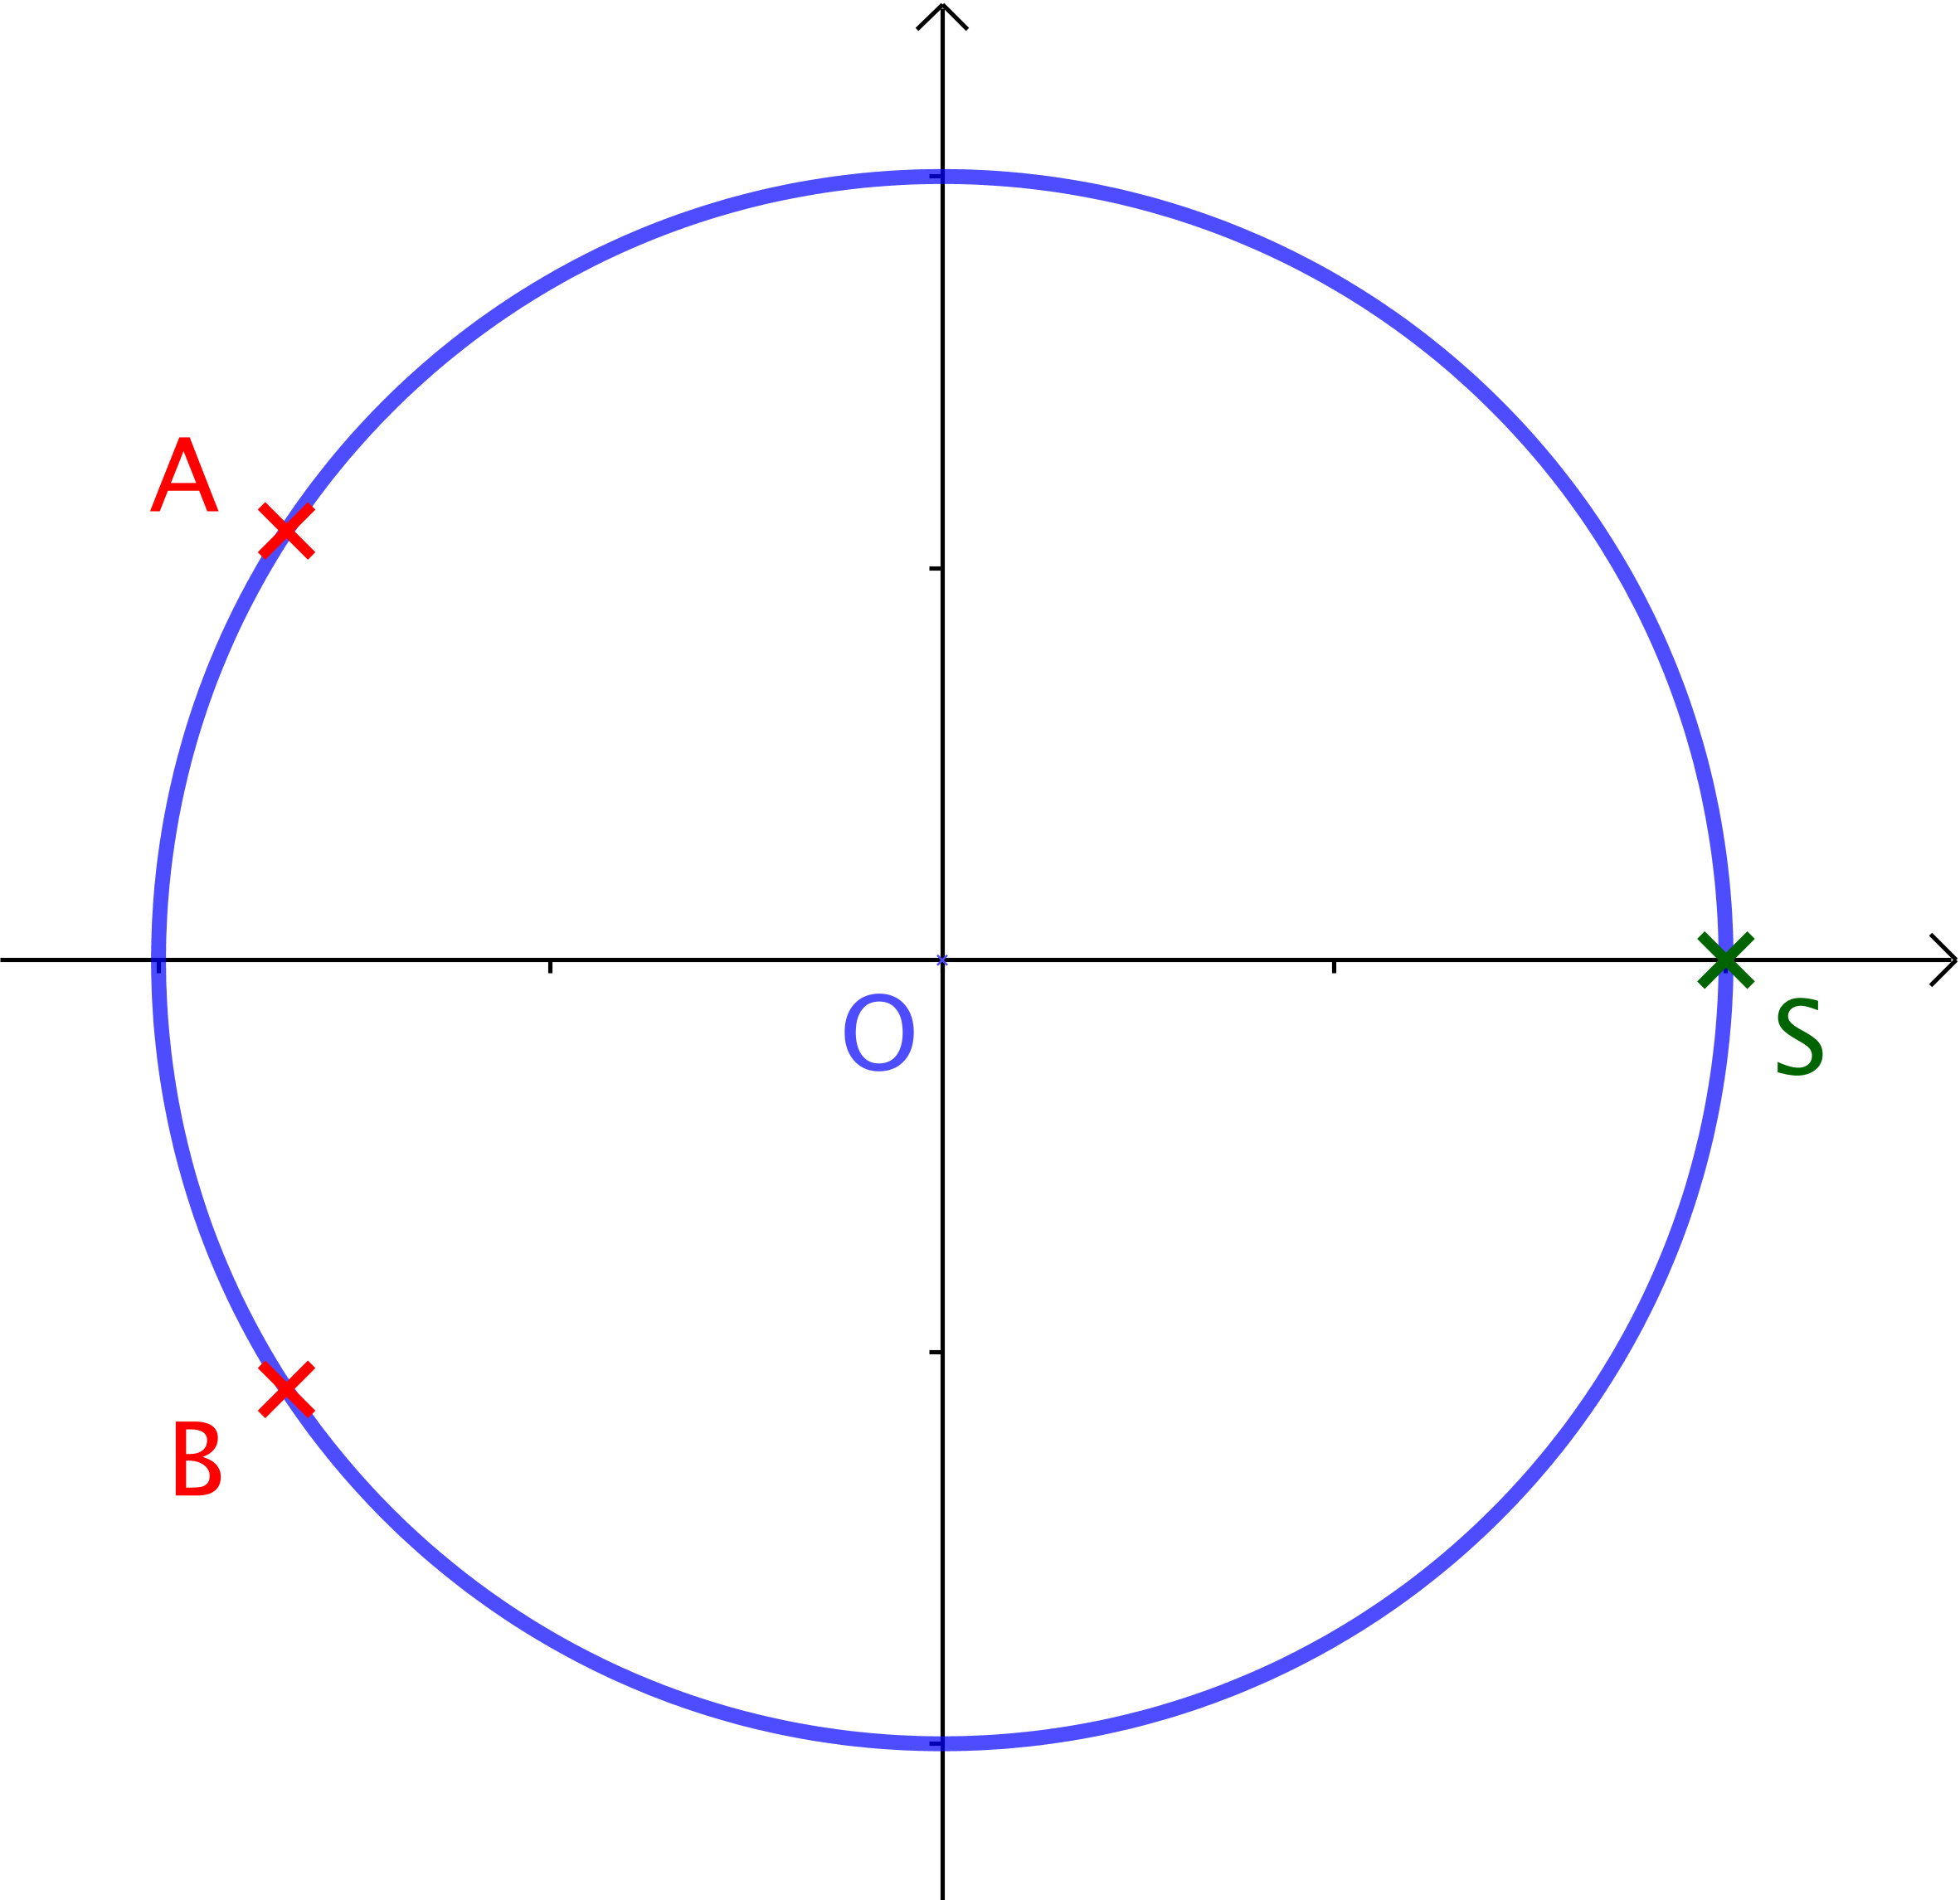
\includegraphics[scale = .75]{addition-on-ellipsis/conjecture/h-sym.png}}

	\columnbreak

	\fbox{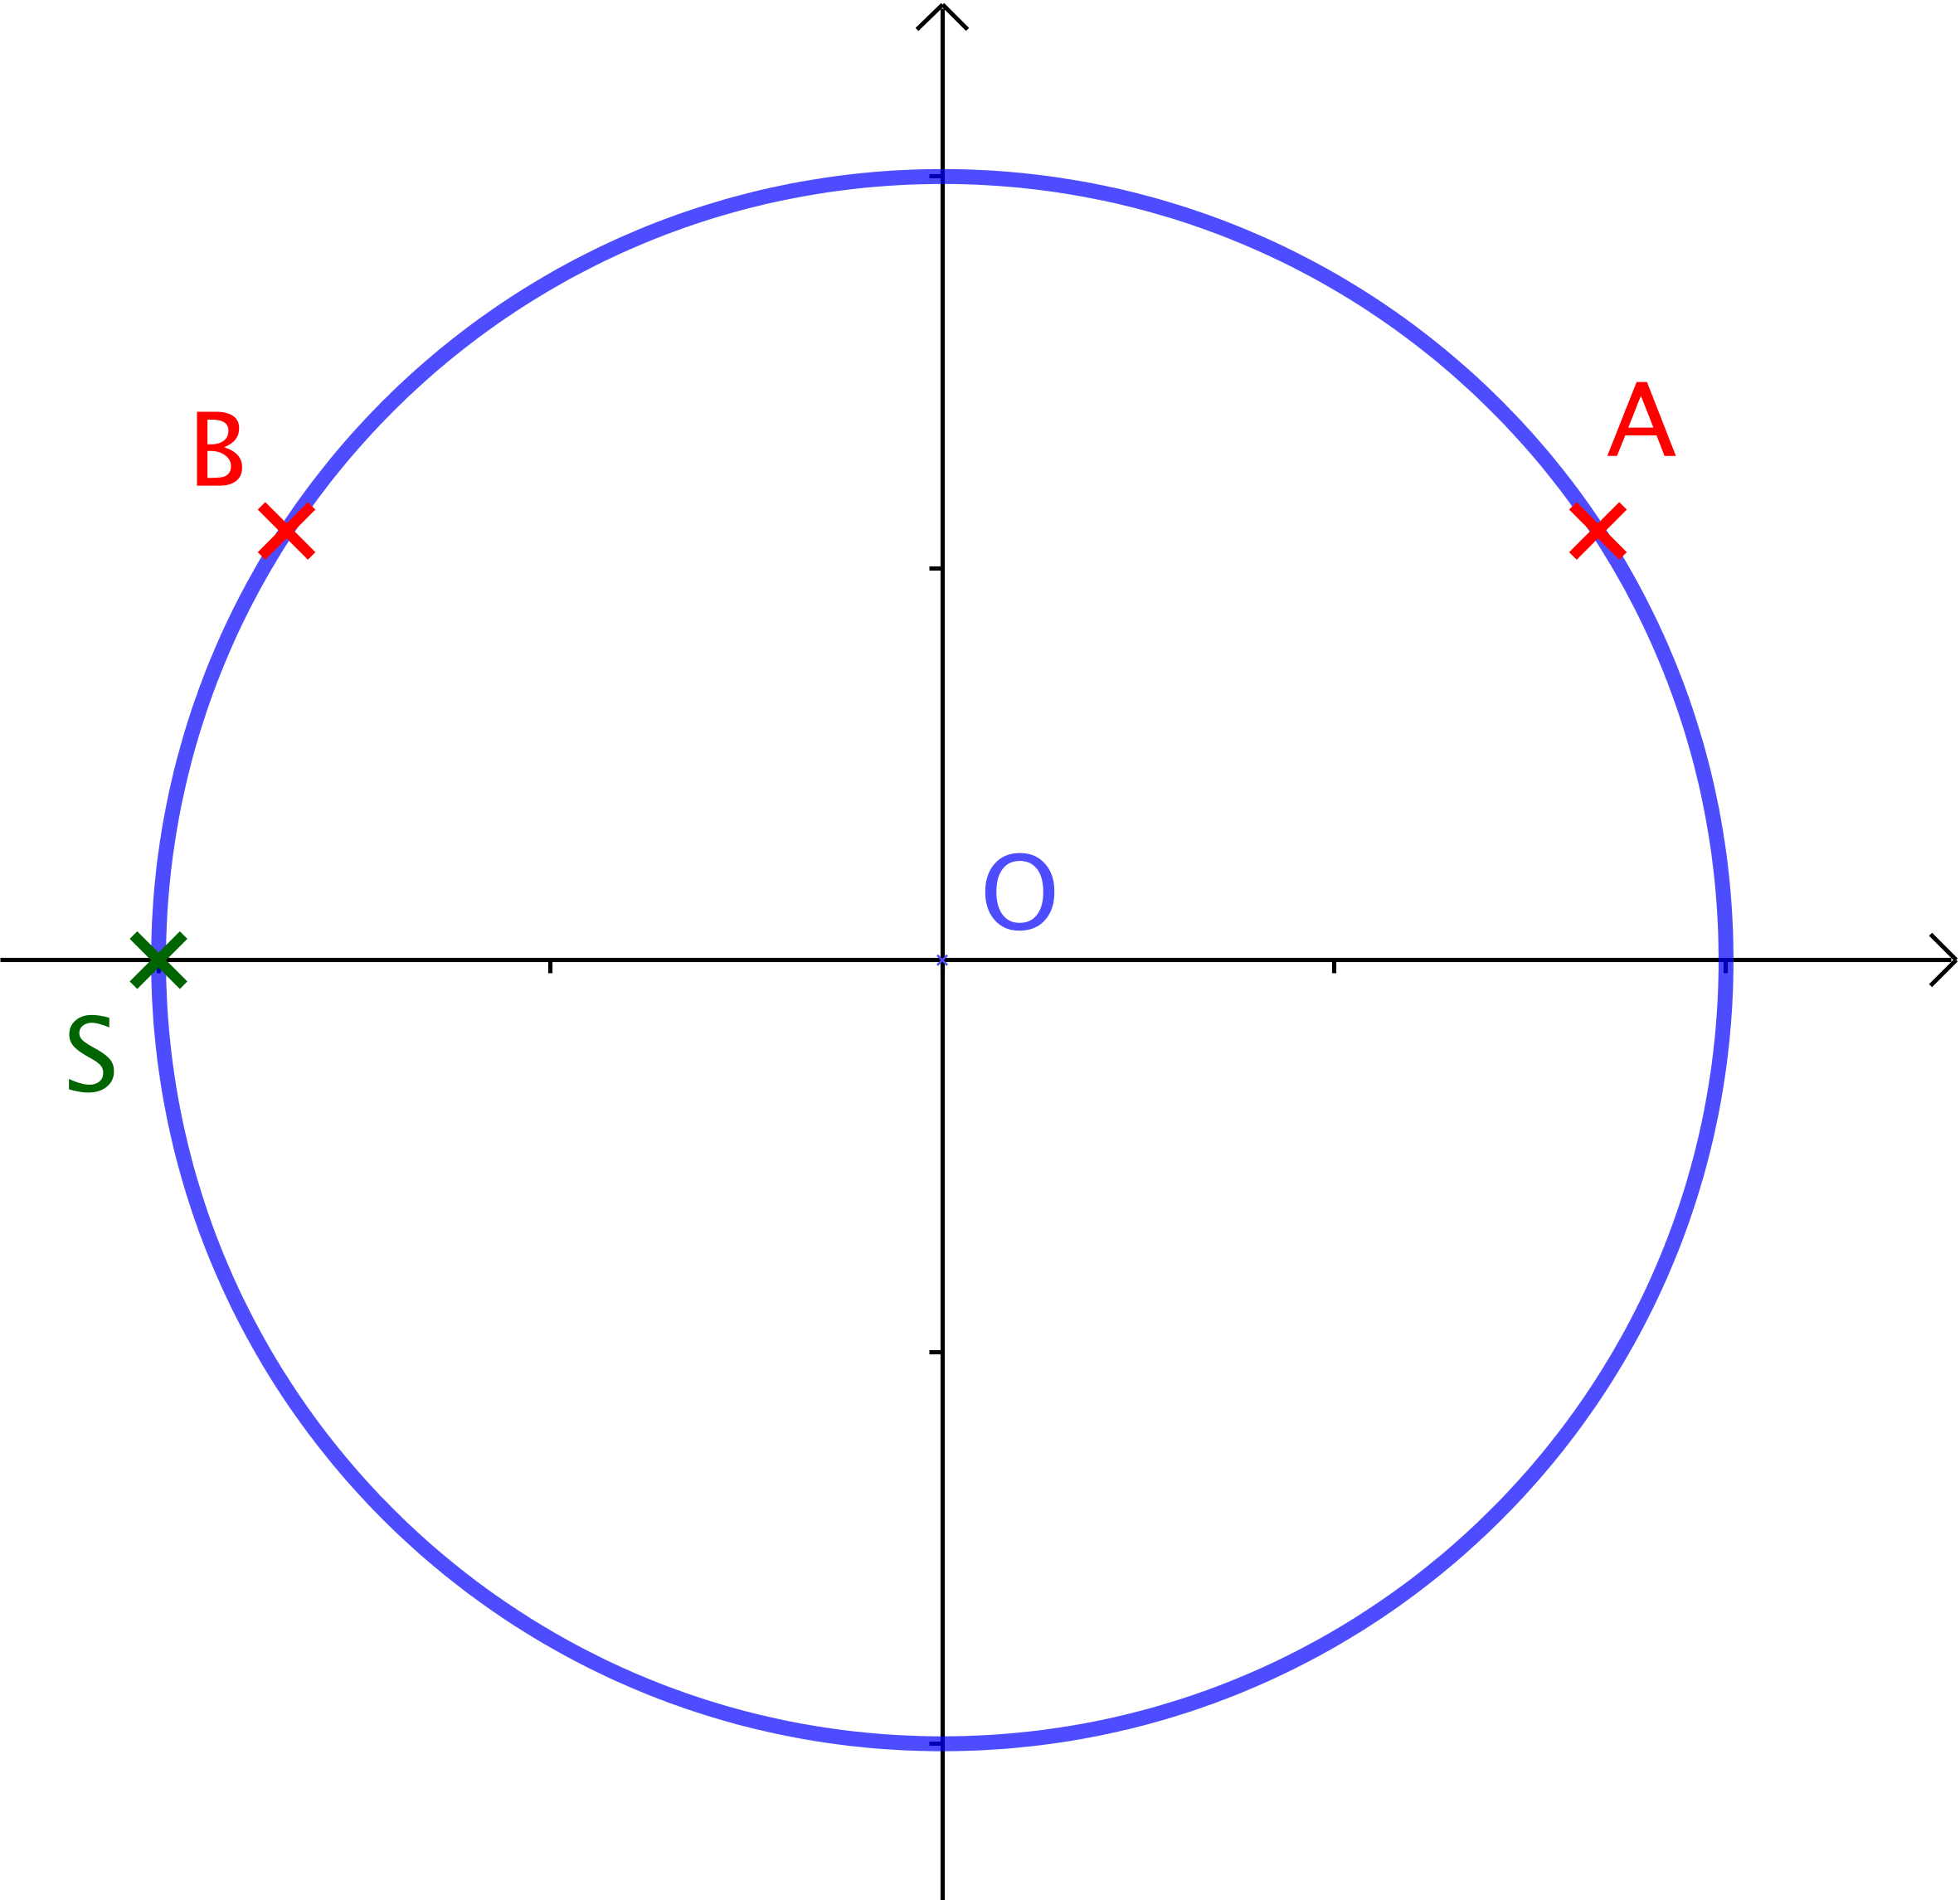
\includegraphics[scale = .75]{addition-on-ellipsis/conjecture/v-sym.png}}
\end{multicols}


\medskip

\begin{multicols}{2}
	\center

	\fbox{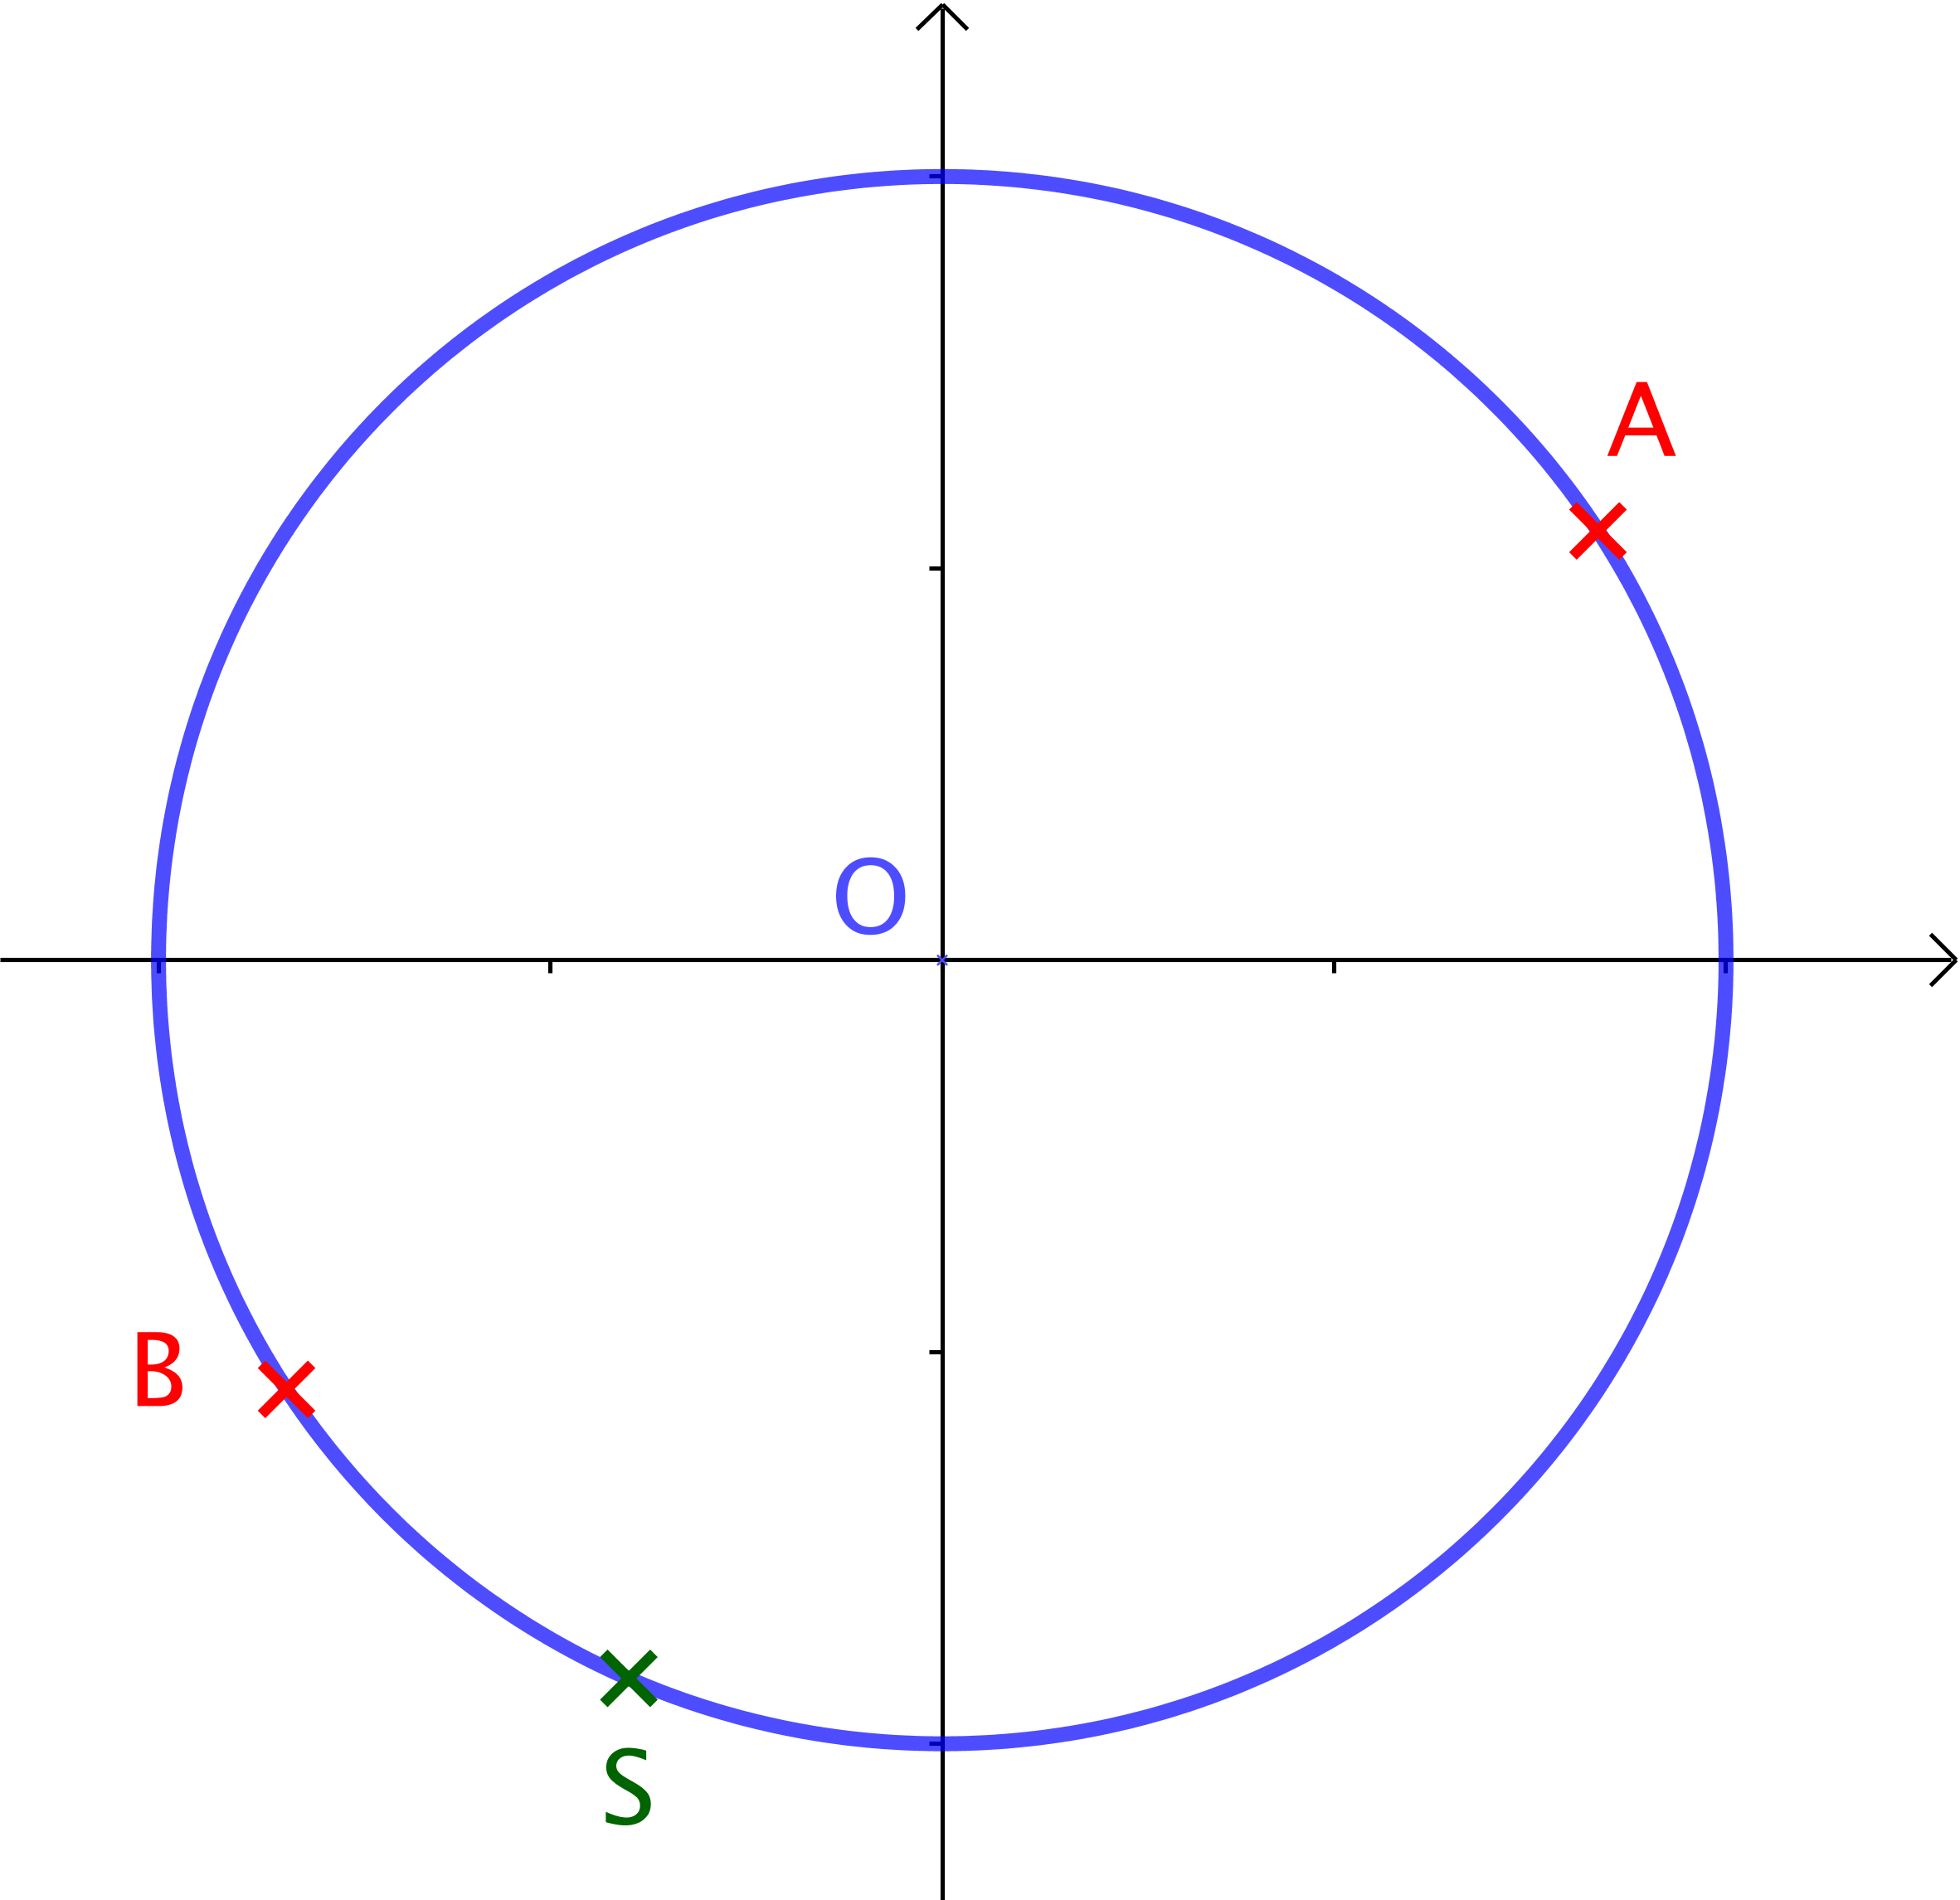
\includegraphics[scale = .75]{addition-on-ellipsis/conjecture/O-sym.png}}

	\columnbreak

	\fbox{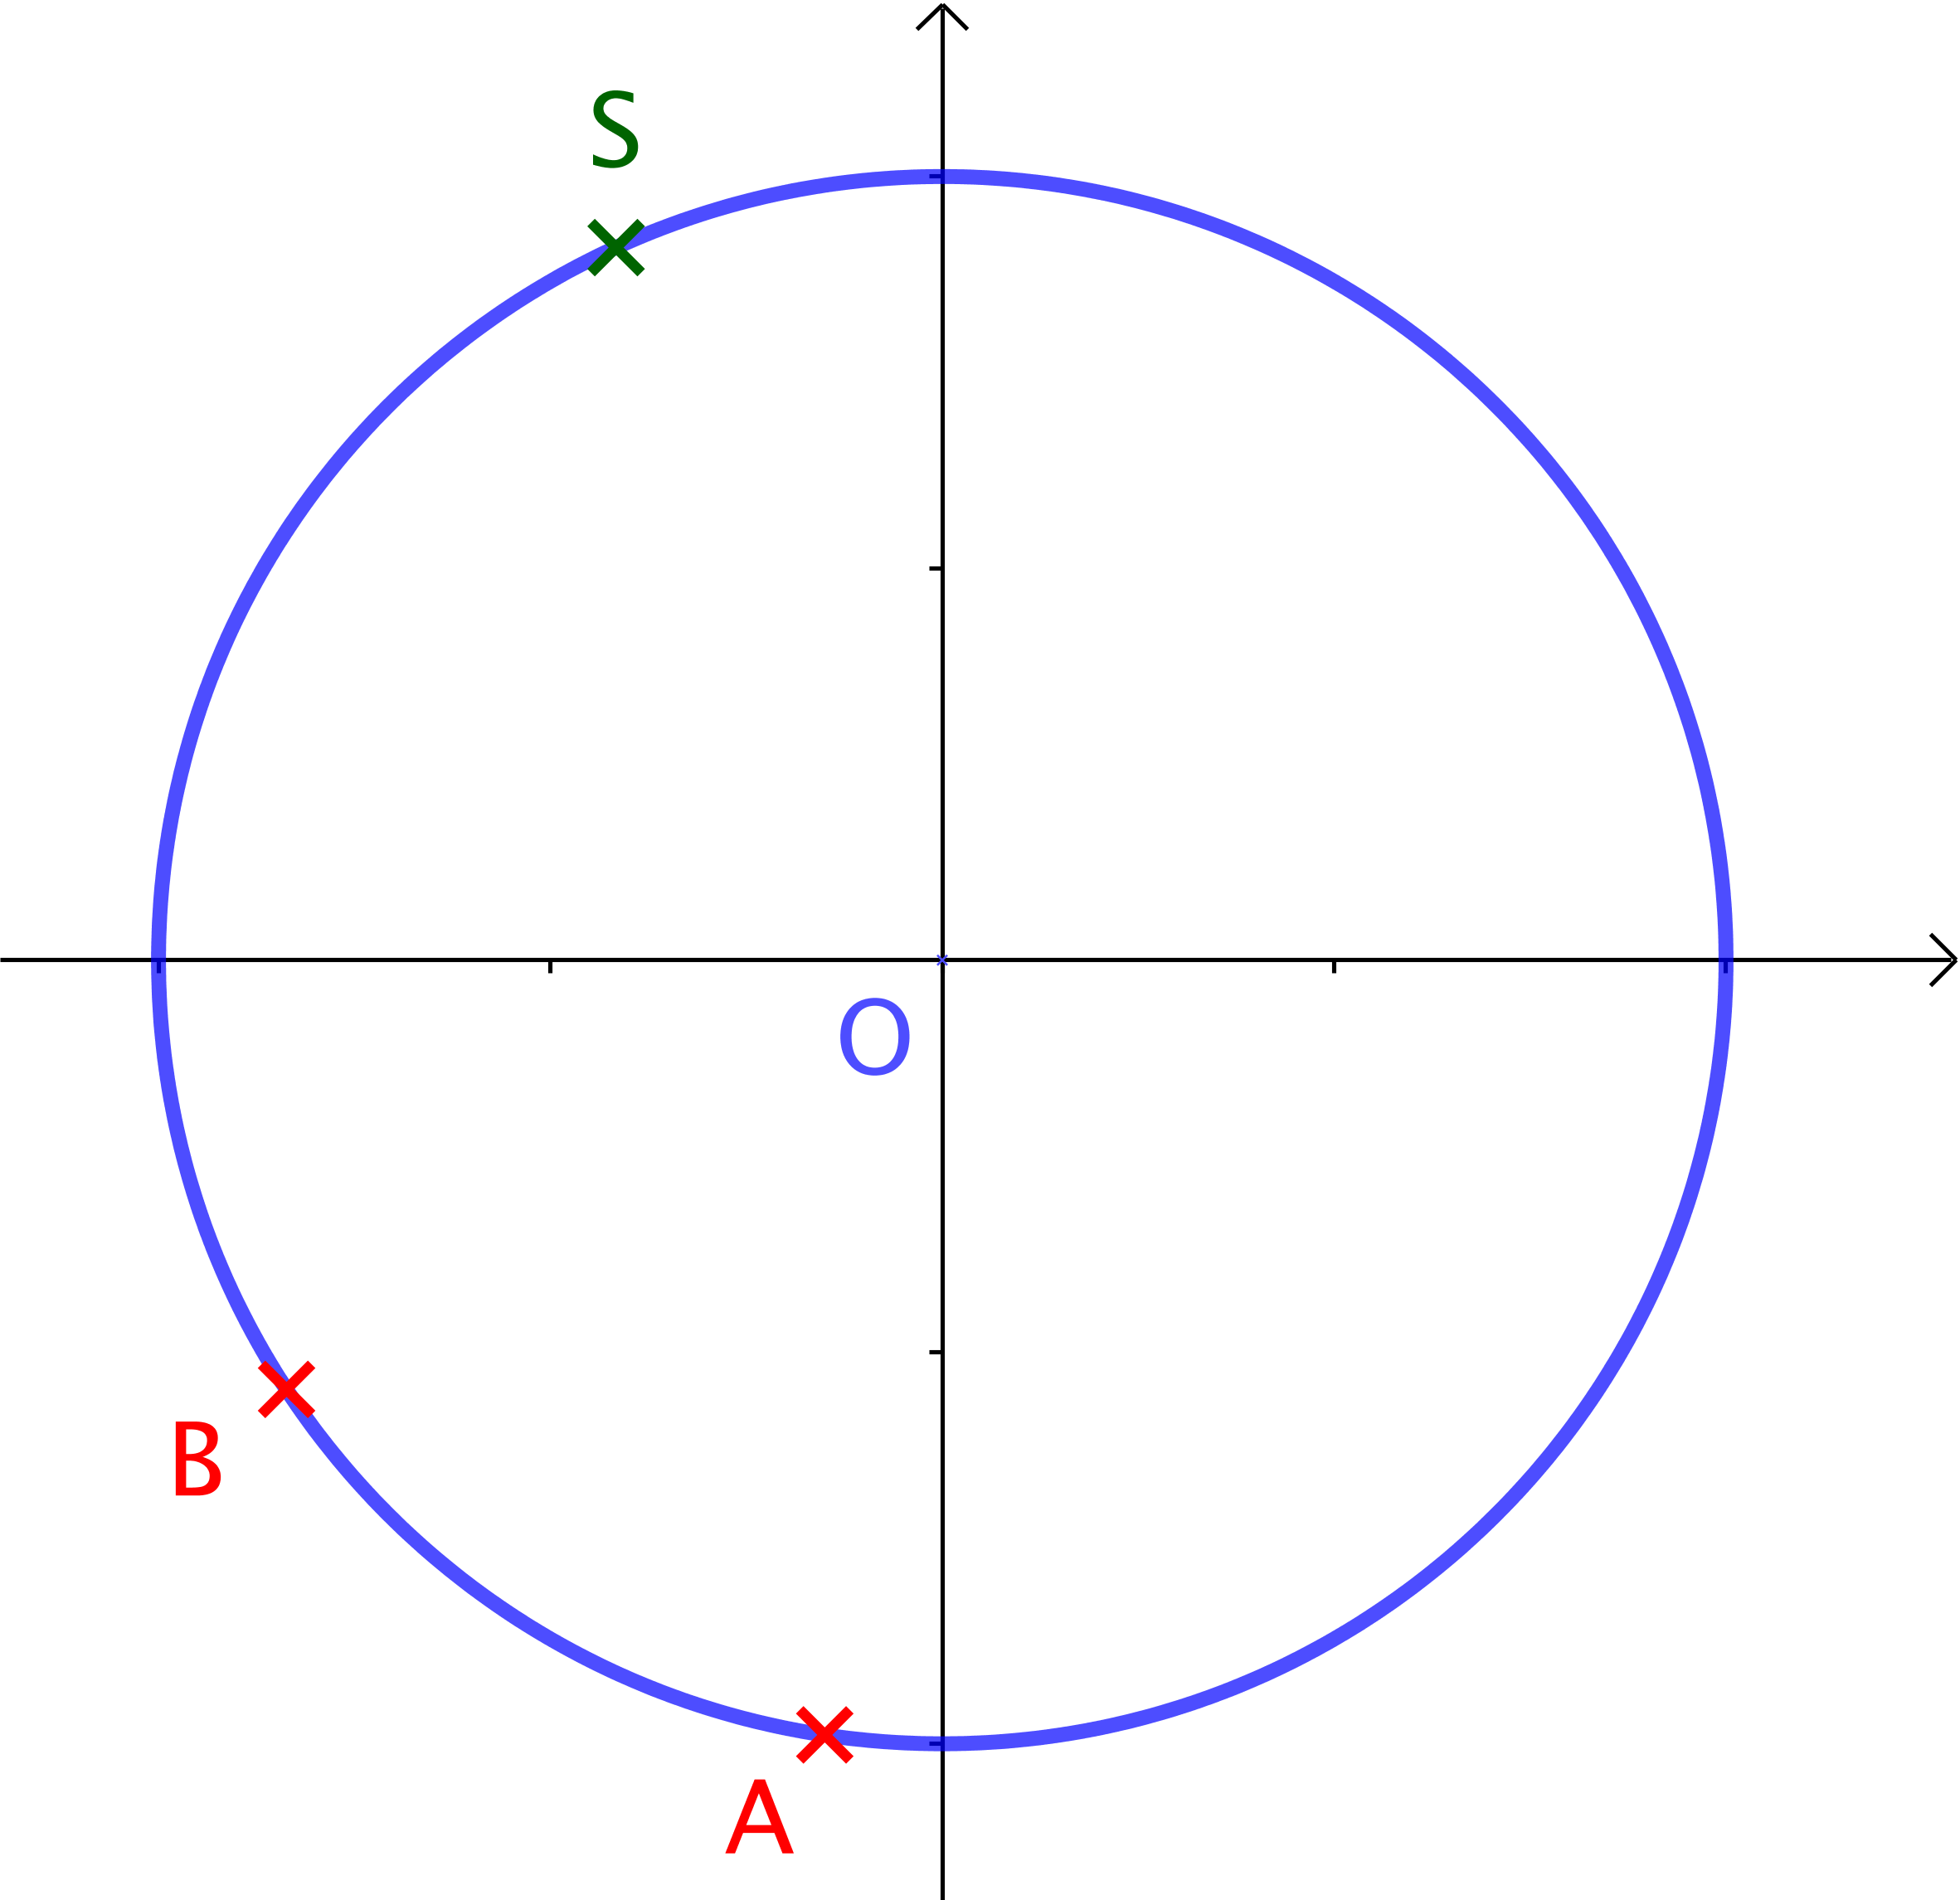
\includegraphics[scale = .75]{addition-on-ellipsis/conjecture/general.png}}
\end{multicols}


\newpage

Pour mieux voir ce qu'il se passe, il suffit de tracer quelques droites. Voici ce que cela donne.

\begin{multicols}{2}
	\center

	\fbox{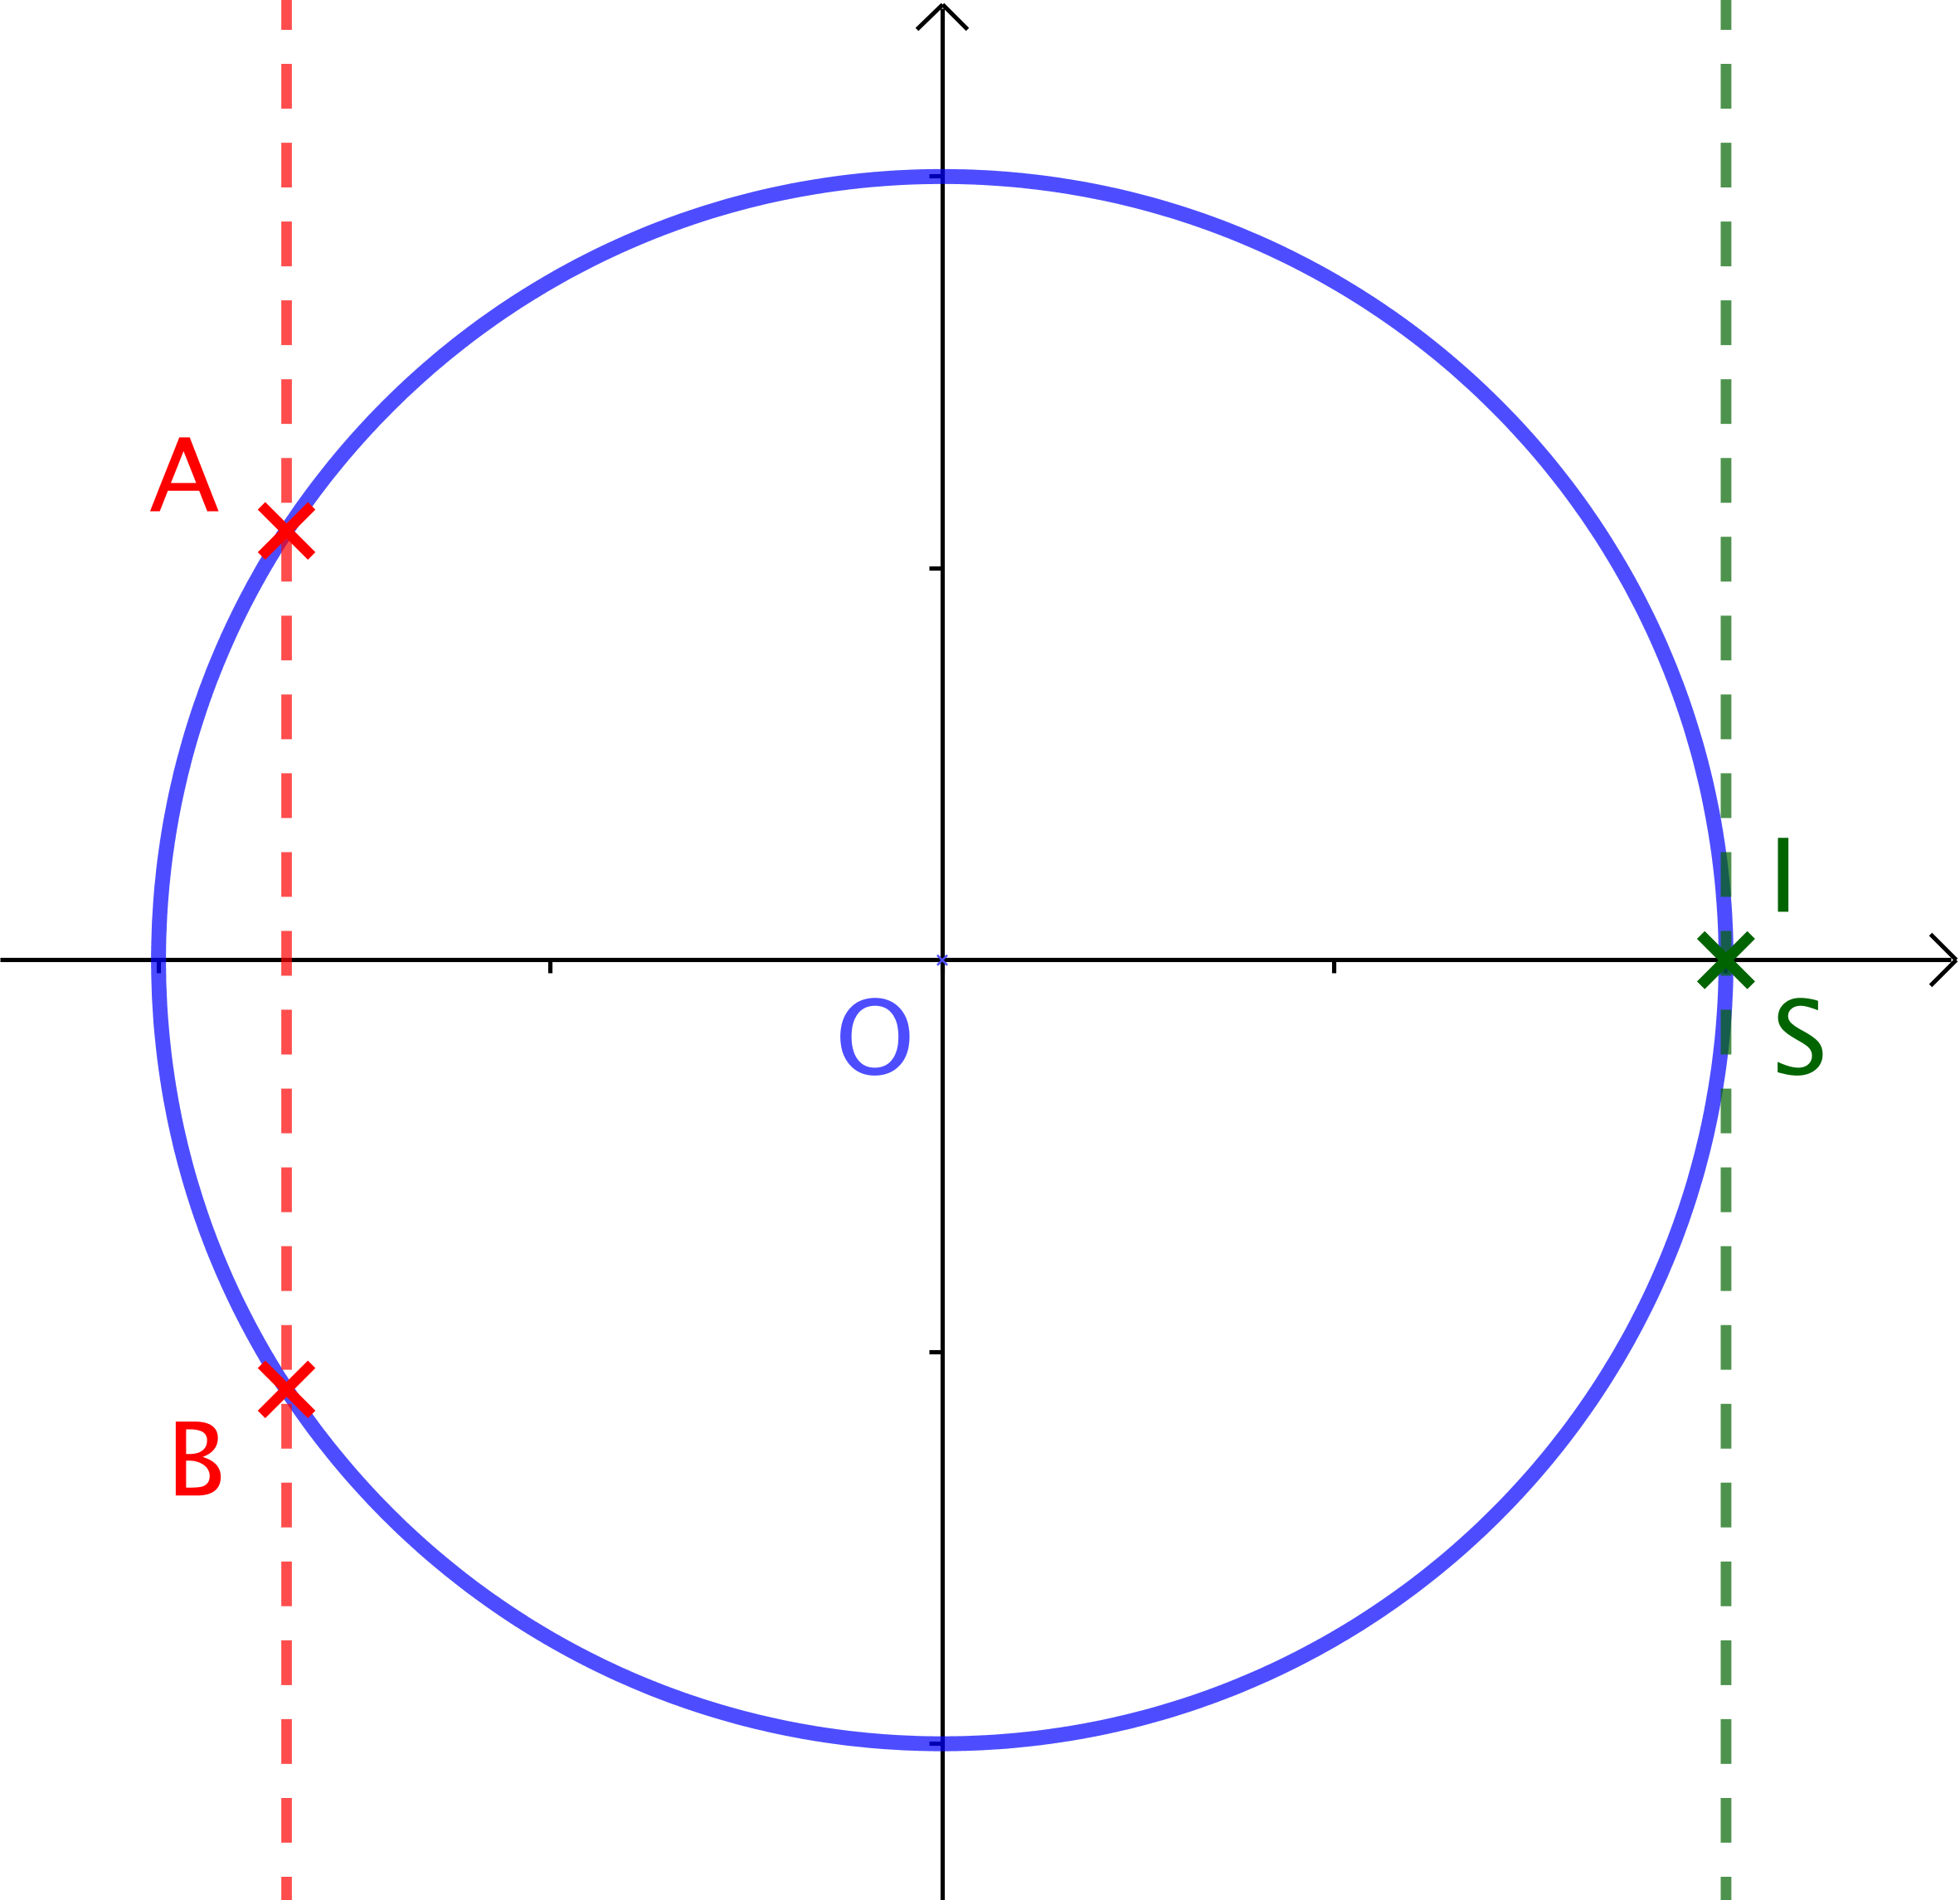
\includegraphics[scale = .75]{addition-on-ellipsis/conjecture/h-sym-with-lines.png}}

	\columnbreak

	\fbox{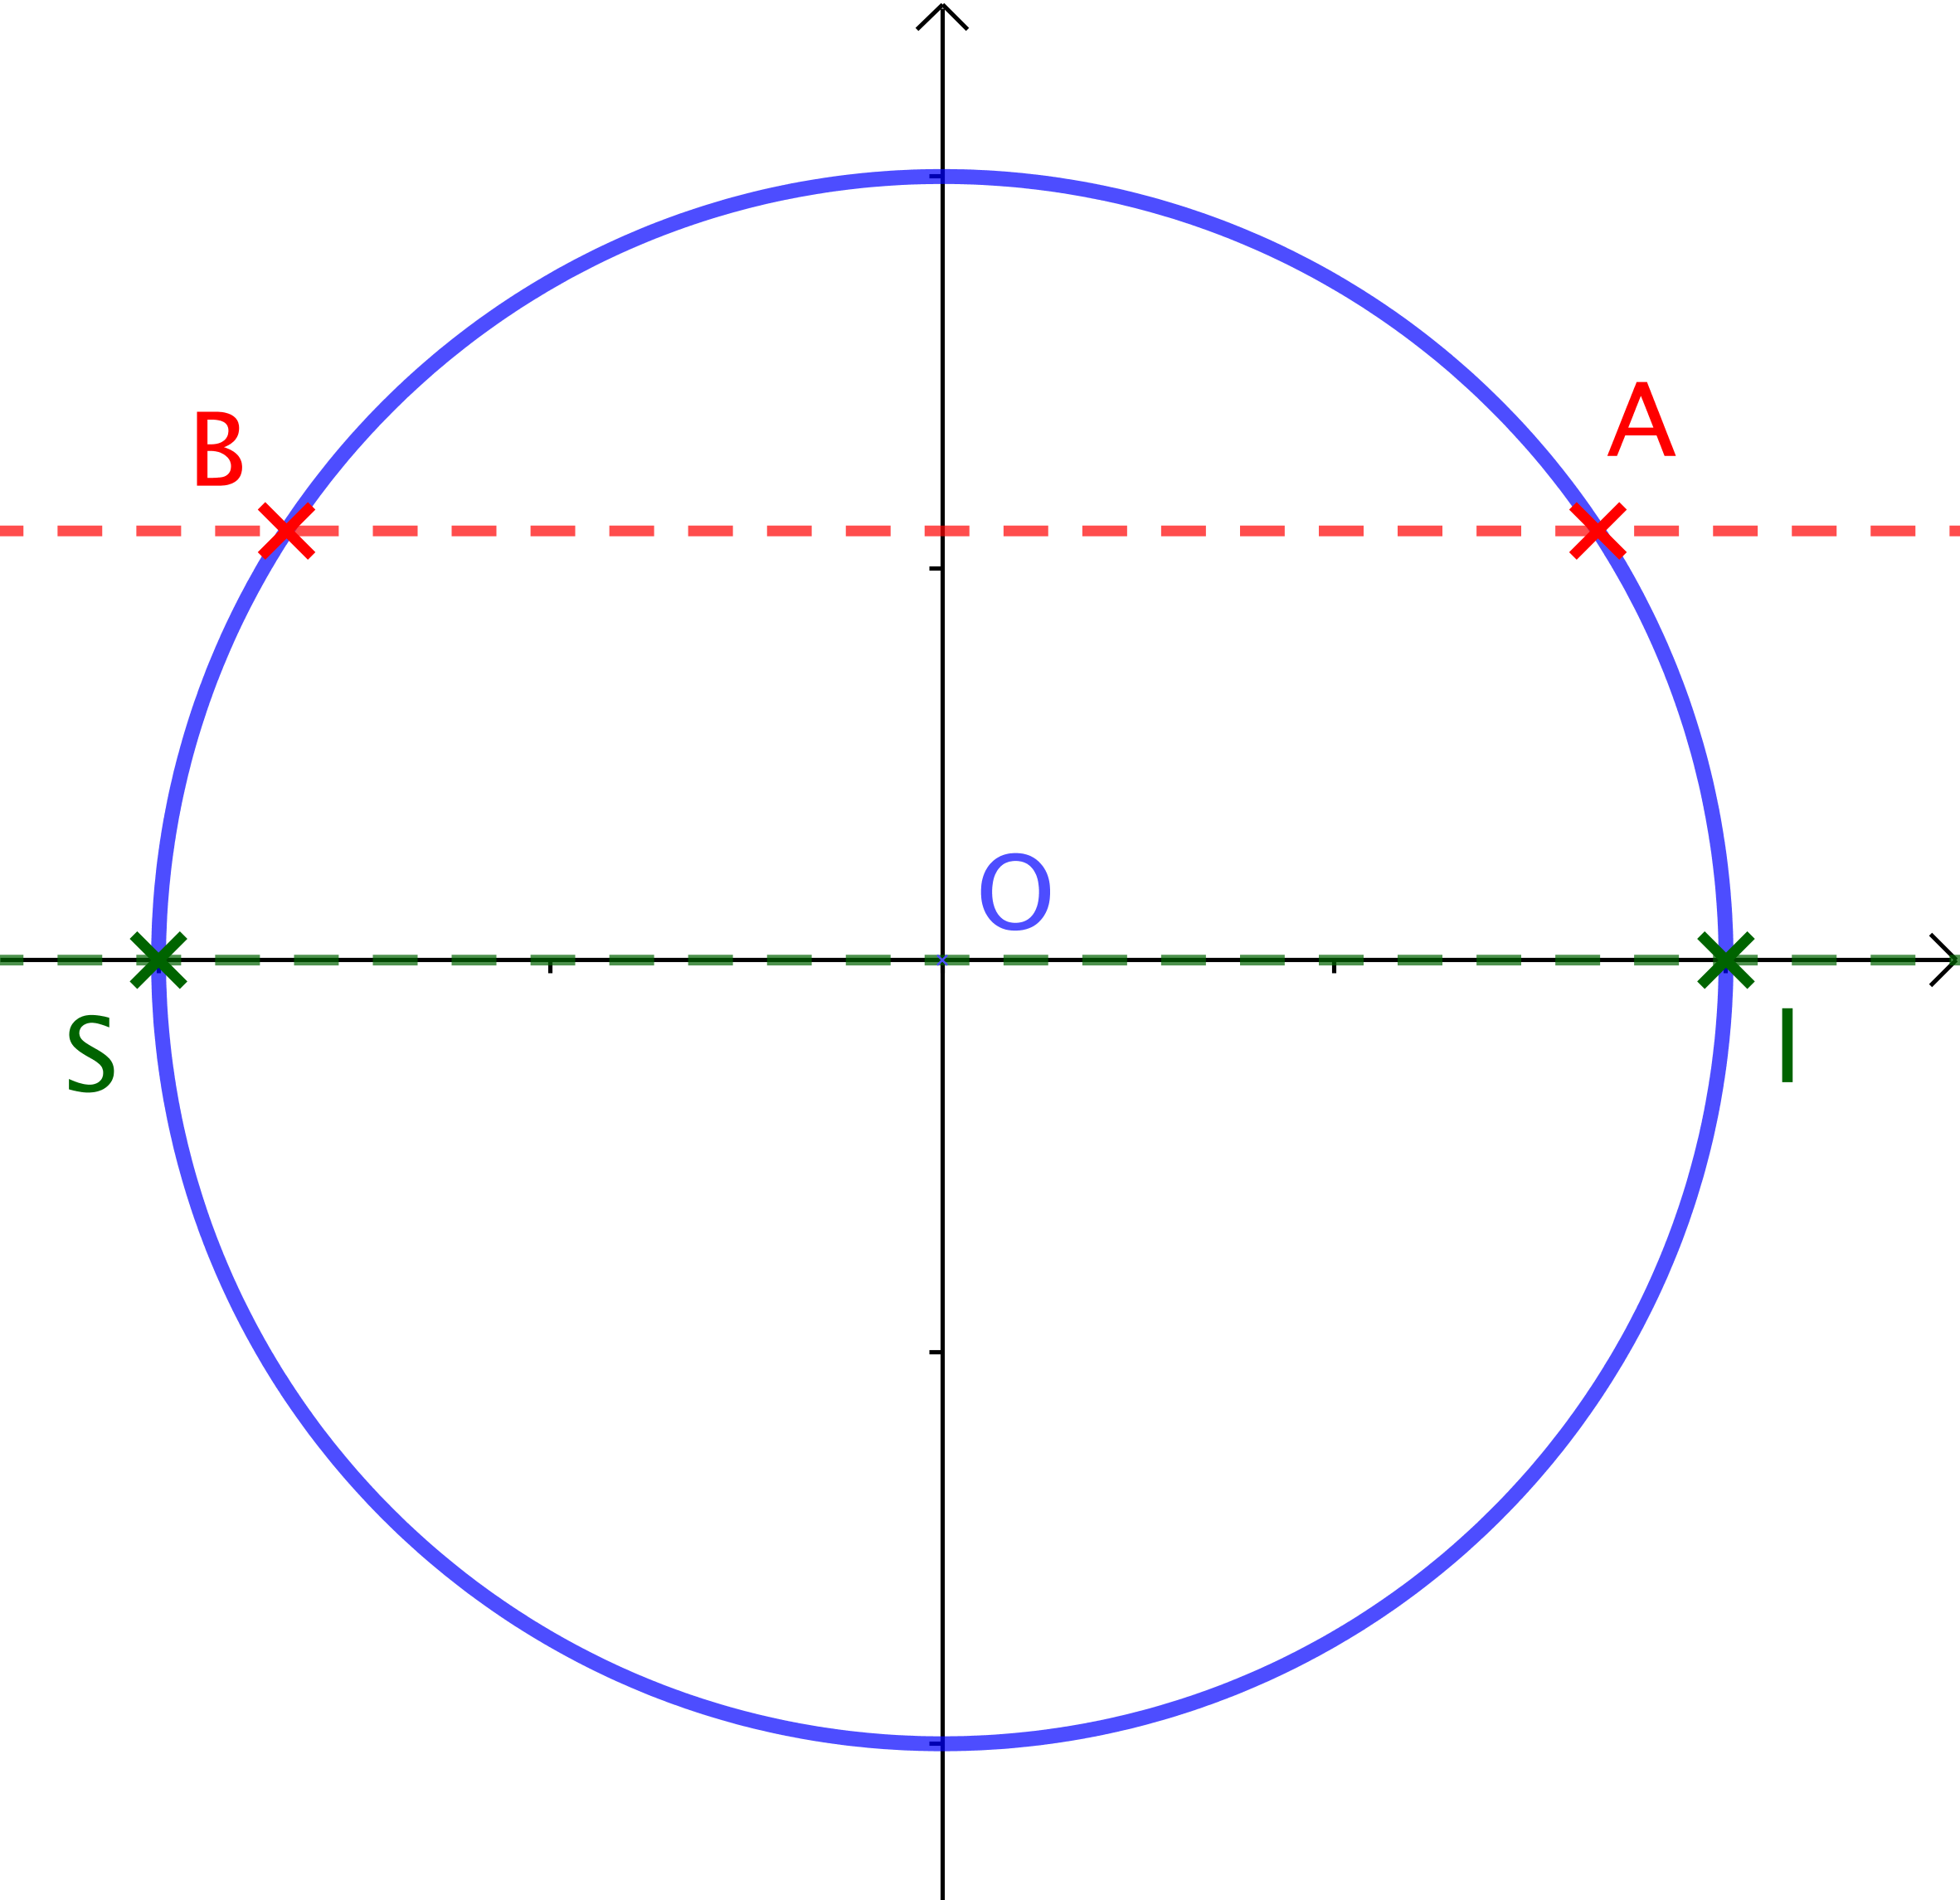
\includegraphics[scale = .75]{addition-on-ellipsis/conjecture/v-sym-with-lines.png}}
\end{multicols}


\medskip

\begin{multicols}{2}
	\center

	\fbox{\includegraphics[scale = .75]{addition-on-ellipsis/conjecture/o-sym-with-lines.png}}

	\columnbreak

	\fbox{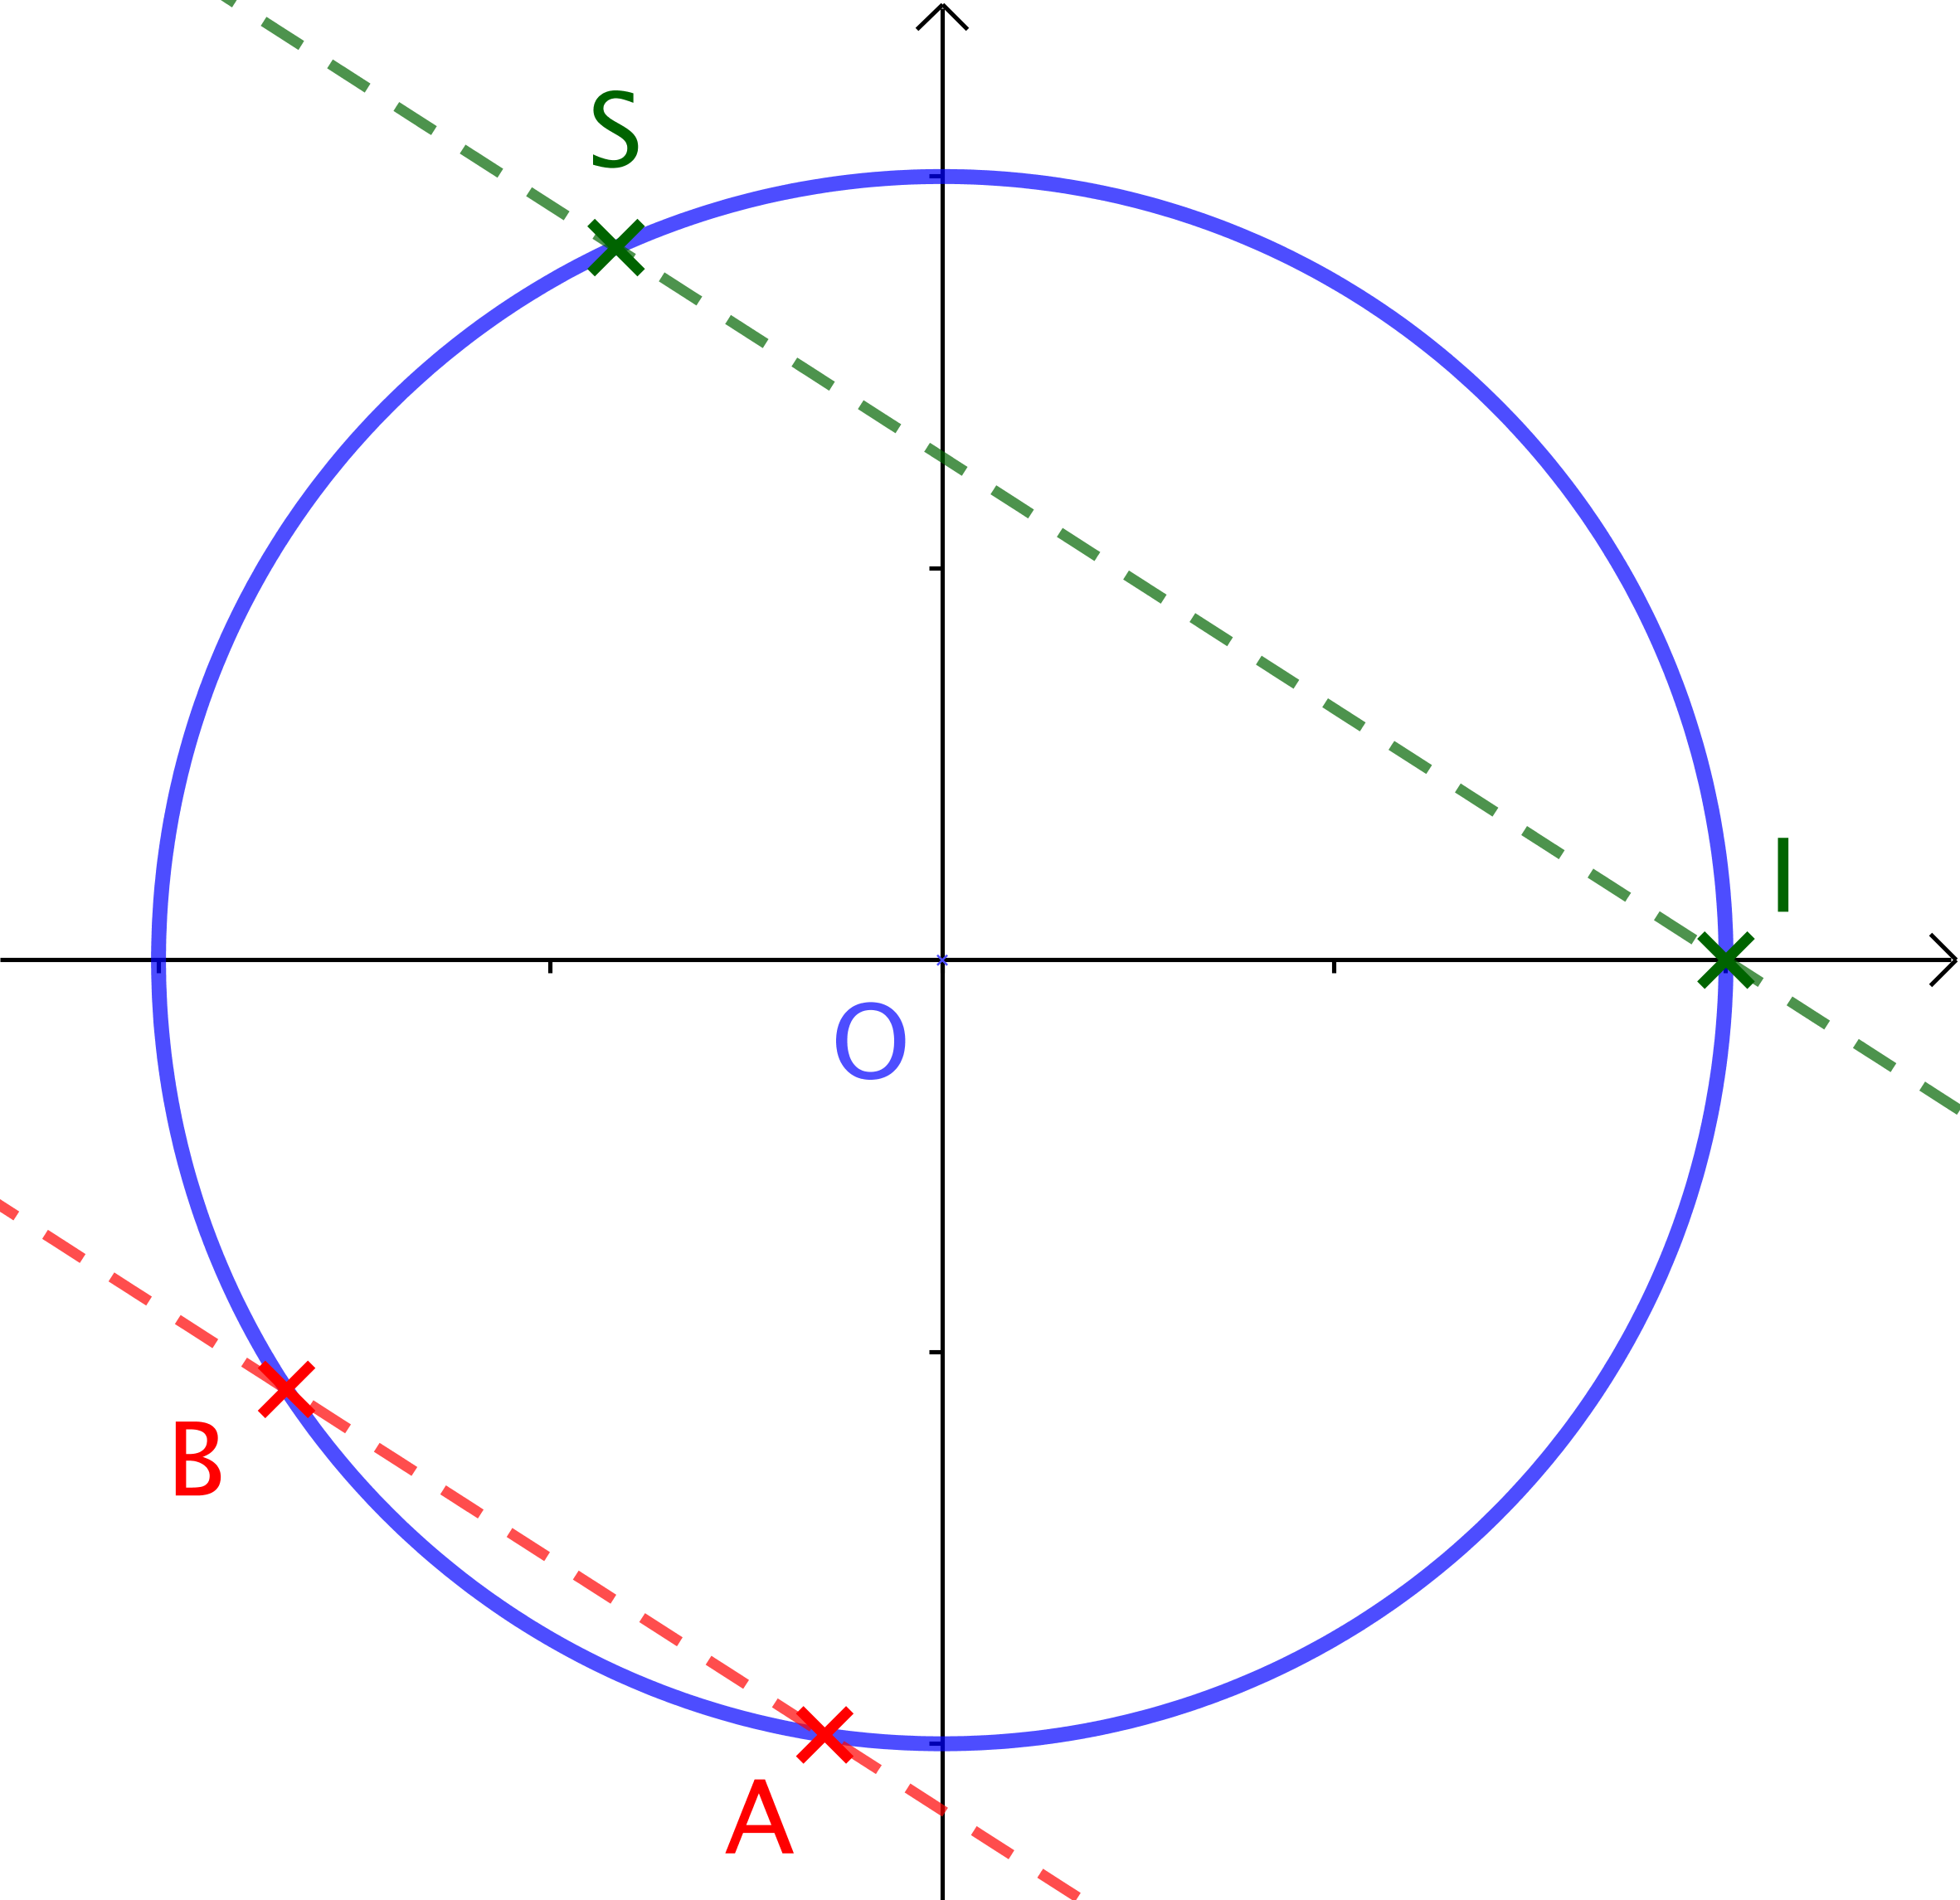
\includegraphics[scale = .75]{addition-on-ellipsis/conjecture/general-with-lines.png}}
\end{multicols}


Il devient évident de conjecturer que le point $S$ se construit géométriquement comme suit.

\begin{enumerate}
	\item \label{point-1} Si $A \neq B$ alors on construit la parallèle à $(AB)$ passant par $I$ . 
	Si cette parallèle n'est pas tangente au cercle alors le point $S$ est le second point d'intersection de cette parallèle avec le cercle, sinon $S = I$ .
	Notons que dans le second cas, c'est à dire si $x_A = x_B$ et $y_A = -y_B$ , alors $S = I$ peut être vu comme un point d'intersection \squote{double}.

	\item Si $A = B$ , on procède comme au point (\ref{point-1}) mais avec la parallèle à la tangente en $A$ au cercle. Intuitivement, cette situation consiste à faire \emph{\og tendre \fg} $A$ vers $B$ 
	\footnote{
		Nous évitons les arguments faisant appel à l'analyse afin de rester dans un cadre géométrique le plus général possible.
	}.
\end{enumerate}


\medskip

Dans ce qui suit nous allons valider cette conjecture de trois façons en allant du plus brutal au plus élégant.

\begin{enumerate}
	\item La 1\iere{} méthode passe assez brutalement via les critères de colinéarité et d'orthogonalité dans un plan.
	
	\item La 2\ieme{} méthode utilise les nombres complexes avec des calculs faciles à mener.
	
	\item La 3\ieme{} méthode, sûrement la plus élégante, est purement géométrique.
\end{enumerate}



% ------------- %


\section{Preuve de la conjecture via le déterminant et le produit scalaire} 

Dans le repère $\paxes{O | I | J}$ supposé orthonormé, $A = (\cos a ; \sin a)$ et $B = (\cos b ; \sin b)$ avec $(a ; b) \in \RR^2$ .
Nous avons alors $S = (\cos(a + b) ; \sin(a + b))$ .
Pour faciliter les calculs, nous posons $A = (c_A ; s_A)$ et $B = (c_B ; s_B)$ de sorte que $S = (c_A c_B - s_A s_B ; c_A s_B + s_A c_B)$ d'après les formules trigonométriques d'addition.


\medskip


\textbf{Cas 1.} \emph{Supposons que $A \neq B$ .}

\medskip

La colinéarité des vecteurs $\vect{AB}$ et $\vect{IS}$ est justifiée par les calculs brutaux suivants \emph{(on pourrait faire appel à un logiciel de calcul formel qui ici peut être utilisé en toute confiance)}.
\begin{flalign*}
	\det\left ( \vect{AB} ; \vect{IS} \right)
		&=
		\left|\begin{NiceArray}{cc} 
			c_B - c_A  &  c_A c_B - s_A s_B - 1 \\ 
			s_B - s_A  &  c_A s_B + s_A c_B
		\end{NiceArray}\right|
		& \\
		&=
		(c_B - c_A)( c_A s_B + s_A c_B)
		-
		(s_B - s_A)(c_A c_B - s_A s_B - 1)
		& \\
		&=
		c_B c_A s_B + s_A c_B^2
		- c_A^2 s_B - c_A s_A c_B
		& \\
		&
		- s_B c_A c_B + s_A s_B^2 + s_B
		+ s_A c_A c_B - s_A^2 s_B - s_A
		& \\
		&=
		s_A c_B^2 - c_A^2 s_B + s_A s_B^2 + s_B - s_A^2 s_B - s_A
		& \\
		&=
		s_A (c_B^2 + s_B^2) - (c_A^2 + s_A^2) s_B + s_B - s_A
		& \\
		&=
		s_A - s_B + s_B - s_A
		& \\
		&=
		0
		& \\
\end{flalign*}

\vspace{-1em}


\textbf{Cas 2.} \emph{Supposons que $A = B$ .}

\medskip

En notant qu'ici $S = (c_A^2 - s_A^2 ; 2 c_A s_A)$ , l'orthogonalité des vecteurs $\vect{OA}$ et $\vect{IS}$ est justifiée par les calculs suivants \emph{(l'usage d'un logiciel de calcul formel serait un peu excessif)}.
\begin{flalign*}
	\dotprod{\vect{OA}}{\vect{IS}}
		&=
		c_A \cdot (c_A^2 - s_A^2 - 1) + s_A \cdot 2 c_A s_A
		& \\
		&=
		c_A \cdot (1 - s_A^2 - s_A^2 - 1) + 2 c_A s_A^2
		& \\
		&=
		- 2 c_A s_A^2 + 2 c_A s_A^2
		& \\
		&=
		0
		& \\
\end{flalign*}

\vspace{-1em}





% ------------- %


\section{Preuve de la conjecture via les complexes}
                        
Travaillons dans le plan complexe associé au repère $\paxes{O | I | J}$ .
Nous posons $z_A = \ee^{\ii a}$ et $z_B = \ee^{\ii b}$ avec $(a ; b) \in \RR^2$ .
Nous avons alors $z_S = \ee^{\ii (a + b)}$ .  


\medskip


\textbf{Cas 1.} \emph{Supposons que $a \not\equiv b \,\, [2\pi]$ , soit $A \neq B$ .}

\medskip

Tout d'abord, nous avons $z_{\vect{AB}} = \ee^{\ii b}- \ee^{\ii a}$ et $z_{\vect{IS}} = \ee^{\ii (a + b)} - 1$. Nous devons trouver un réel $k \in \RR$ tel que $z_{\vect{IS}} = k z_{\vect{AB}}$ . Dans la suite, nous noterons $s = a + b$ . Nous avons alors :
\begin{flalign*}
	z_{\vect{IS}} 
		&= \ee^{\ii s} - 1
		& \\
		&= \ee^{\ii s / 2} \left( \ee^{\ii s / 2} - \ee^{- \ii s / 2} \right)
		& \\
		&= \ee^{\ii s / 2} \cdot 2 \ii \sin(0,5 s)
		& \\
		&= 2 \ii \sin(0,5 s) \ee^{\ii s / 2}
		& \\
\end{flalign*}

\vspace{-1em}

A l'aide de la même technique classique précédente, notant $d = b - a$, nous obtenons :
\begin{flalign*}
	z_{\vect{AB}} 
		&= \ee^{\ii b}- \ee^{\ii a}
		& \\
		&= \ee^{\ii a} \left( \ee^{\ii d} - 1 \right)
		& \\
		&= \ee^{\ii a} \cdot 2 \ii \sin(0,5 d) \ee^{\ii d / 2}
		& \\
		&= 2 \ii \sin(0,5 d) \ee^{\ii s / 2}
		& \text{En effet, $d + 2 a = s$.} \\
\end{flalign*}

\vspace{-1em}


Comme $d \not\equiv 0 \,\, [2\pi]$ par hypothèse, soit de façon équivalente $0,5 d \not\equiv 0 \,\, [\pi]$ , nous avons finalement $z_{\vect{IS}} = k z_{\vect{AB}}$ où $k = \frac{\sin(0,5 s)}{\sin(0,5 d)} \in \RR$ .



\bigskip

\textbf{Cas 2.} \emph{Supposons que $a \equiv b \,\, [2\pi]$ , soit $A = B$ .}

\medskip

Nous devons prouver l'orthogonalité des vecteurs $\vect{OA}$ et $\vect{IS}$ avec ici $z_S = \ee^{2 \ii a}$ .
Ceci découle de la nullité de la partie réelle du produit suivant
\footnote{
	Se souvenir que 
	$(x + \ii y) \, \overline{(x' + \ii y')} = xx' + yy' +\ii (x'y - xy')$ .
	Notez que cette identité est un deux-en-un contenant le produit scalaire et le déterminant des vecteurs $\vect{u}$ et $\vect{v}$ d'affixes complexes respectives $(x + \ii y)$ et $(x' + \ii y')$ .
	Si $\vect{u} \neq \vect{0}$ et $\vect{v} \neq \vect{0}$ ,
	la notation exponentielle nous donne sans effort que
	$\cos \theta = \frac{\dotprod{\vect{u}}{\vect{v}}}{\norm{\vect{u}} \cdot \norm{\vect{v}}}$
	et
	$\sin \theta = \frac{\det\left ( \vect{u} ; \vect{v} \right)}{\norm{\vect{u}} \cdot \norm{\vect{v}}}$
	où $\theta$ est une mesure en radians de l'angle orienté $\angleorient{\vect{u}}{\vect{v}}$.
}.
\begin{flalign*}
	z_{\vect{OA}} \,\, \overline{z_{\vect{IS}} \vphantom{T}}
		&= \ee^{\ii a} \, \overline{\left( \ee^{2 \ii a} - 1 \right)}
		& \\
		&= \ee^{\ii a} \, \left( \ee^{- 2 \ii a} - 1 \right)
		& \\
		&= \ee^{- \ii a} - \ee^{\ii a}
		& \\
		&= 2 \ii \sin a
		& \\
\end{flalign*}

\vspace{-1em}



% ------------- %


\section{Preuve de la conjecture via la si belle géométrie} 

Bien qu'un peu longue à rédiger, la preuve présentée ici est presque évidente par simple lecture des dessins bien codés ci-après. En tout cas, elle s'explique très vite à l'oral sans faire appel à aucun calcul !


\bigskip


\textbf{Cas 1.} \emph{Supposons que $A = I$ ou $B = I$ .}

\medskip

Par symétrie des rôles, on peut juste traiter la situation où $A = I$ . Dans ce cas, $\vangleorient{OI}{OA}$ est nul d'où $\vangleorient{OI}{OS} = \vangleorient{OI}{OB}$ soit $B = S$ . On conclut comme suit.

\begin{enumerate}
	\item Si $A \neq B$ alors la parallèle à $(AB)$ passant par $I = A$ n'est autre que $(AB)$ .
	Suivant que cette parallèle est tangente ou non au cercle, on aura bien à chaque fois $S = B$ .

	\item Si $A = B$ , on raisonne de même avec la parallèle à la tangente en $A$ au cercle.
\end{enumerate}


% -------------- %


\bigskip


\textbf{Cas 2.} \emph{Supposons que $A \neq B$ avec $A \neq I$ et $B \neq I$ .}

\medskip

Nous avons donc une situation du type suivant où sont indiqués des angles très intéressants comme nous allons le constater tout de suite.

\smallskip
\begin{center}
	\fbox{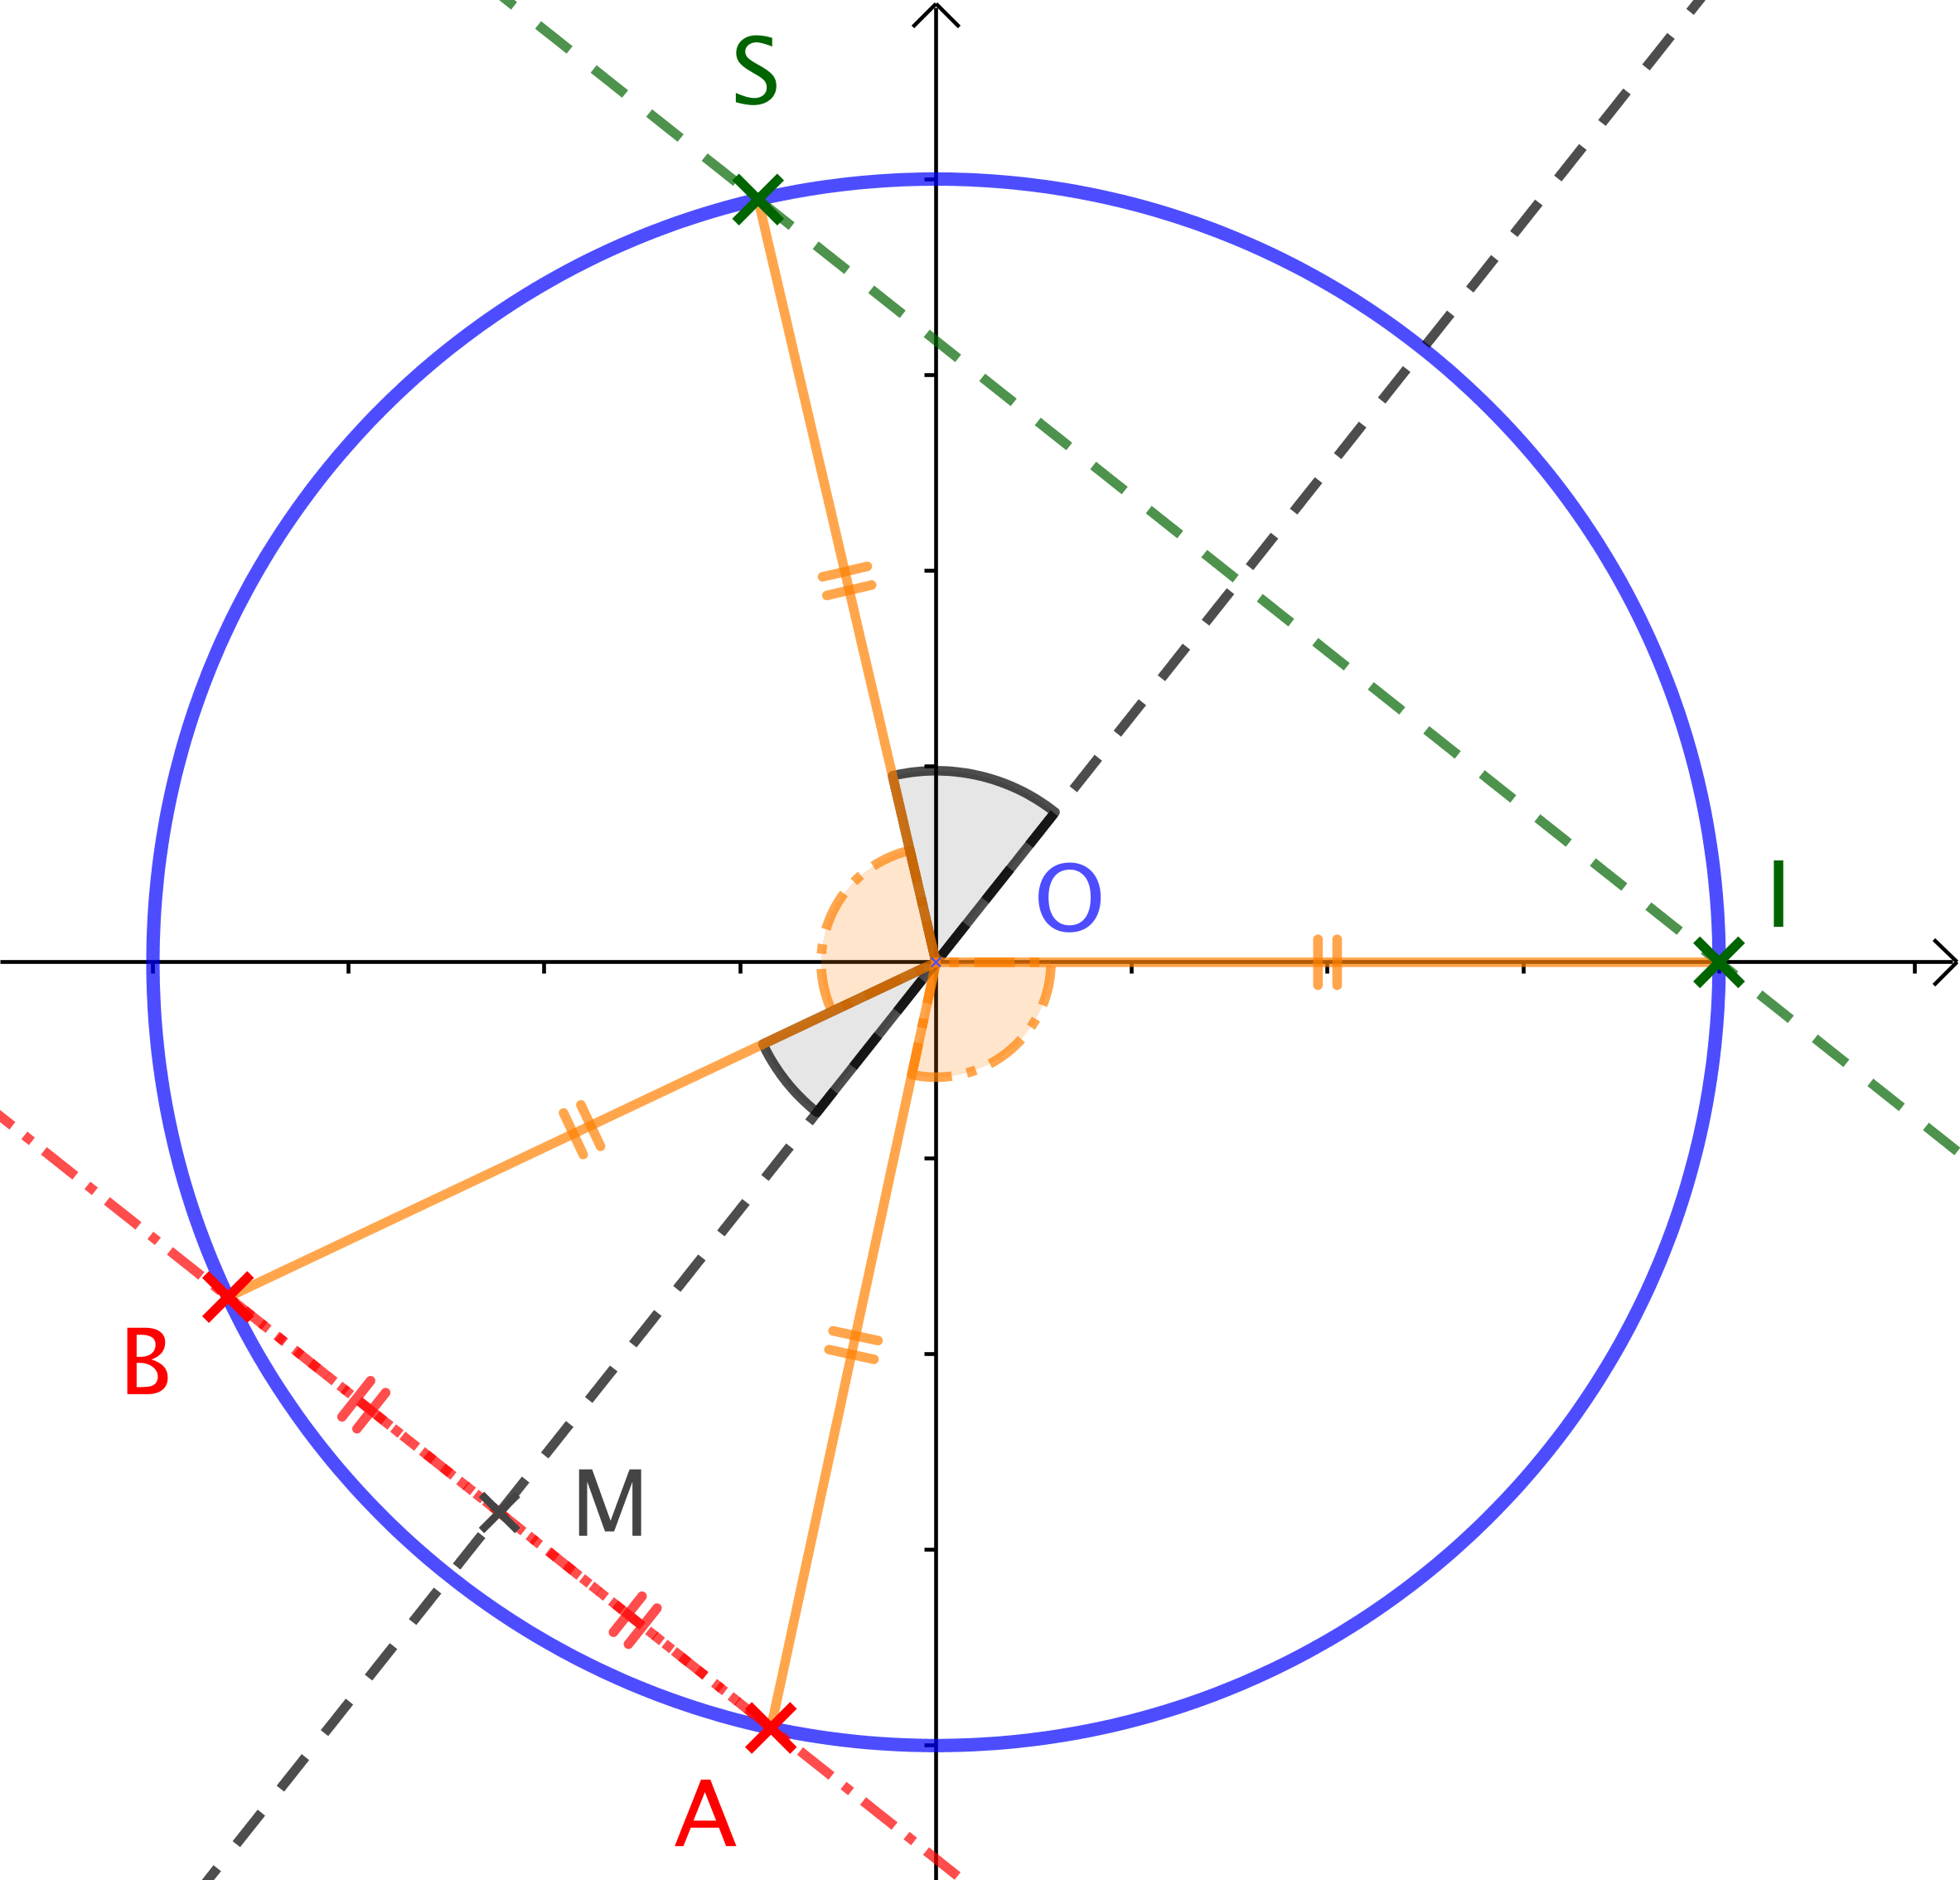
\includegraphics[scale = .75]{addition-on-ellipsis/proof/rotation-A-not-B.png}}
\end{center}
\smallskip

Comme 
$\angleorient{\vect{OB}}{\vect{OS}}
= \angleorient{\vect{OB}}{\vect{OI}}
+ \angleorient{\vect{OI}}{\vect{OS}}$
et
$\angleorient{\vect{OI}}{\vect{OS}}
= \angleorient{\vect{OI}}{\vect{OA}}
+ \angleorient{\vect{OI}}{\vect{OB}}$ 
par définition de $S$ , nous avons :
$\angleorient{\vect{OB}}{\vect{OS}}
= \angleorient{\vect{OI}}{\vect{OA}}$
.


\smallskip

Ensuite, notant $M$ le milieu de $[AB]$ , la médiane $(OM)$ est aussi une bissectrice du triangle $BOA$ isocèle en $O$ de sorte que
$\angleorient{\vect{OM}}{\vect{OB}} 
= - \angleorient{\vect{OM}}{\vect{OA}}$ 
.


\smallskip

Notant $\Pi$ l'angle plat, nous avons alors :
\begin{flalign*}
	\angleorient{\vect{MO}}{\vect{OS}}
		&= \angleorient{\vect{MO}}{\vect{OM}} 
		 + \angleorient{\vect{OM}}{\vect{OB}}
		 + \angleorient{\vect{OB}}{\vect{OS}}
		& \\
		&= \Pi
		 - \angleorient{\vect{OM}}{\vect{OA}}
		 + \angleorient{\vect{OI}}{\vect{OA}}
		& \\
		&= \Pi
		 + \angleorient{\vect{OA}}{\vect{OM}}
		 + \angleorient{\vect{OI}}{\vect{OA}}
		& \\
		&= \Pi
		 + \angleorient{\vect{OI}}{\vect{OM}}
		& \\
		&= \angleorient{\vect{OI}}{- \, \vect{OM}}
		& \\
		&= \angleorient{\vect{OI}}{\vect{MO}}
		& \\
		&= - \angleorient{\vect{MO}}{\vect{OI}}
		& \\
\end{flalign*}

\vspace{-1.5em}


Comme
$\angleorient{\vect{MO}}{\vect{OS}} 
= - \angleorient{\vect{MO}}{\vect{OI}}$ ,
la droite $(OM)$ est aussi une bissectrice du triangle $SOI$ isocèle en $O$ .
Or la bissectrice issue du sommet principal d'un triangle isocèle est aussi une hauteur d'où $(OM) \,\bot\, (AB)$ et $(OM) \,\bot\, (SI)$ puis $(AB) \,/\!/\, (SI)$ comme souhaité.



% -------------- %


\bigskip

\textbf{Cas 3.} \emph{Supposons que $A = B \neq I$ .}

\medskip

Tout est dans le dessin suivant ou presque. Nous allons rédiger cela proprement.

\smallskip
\begin{center}
	\fbox{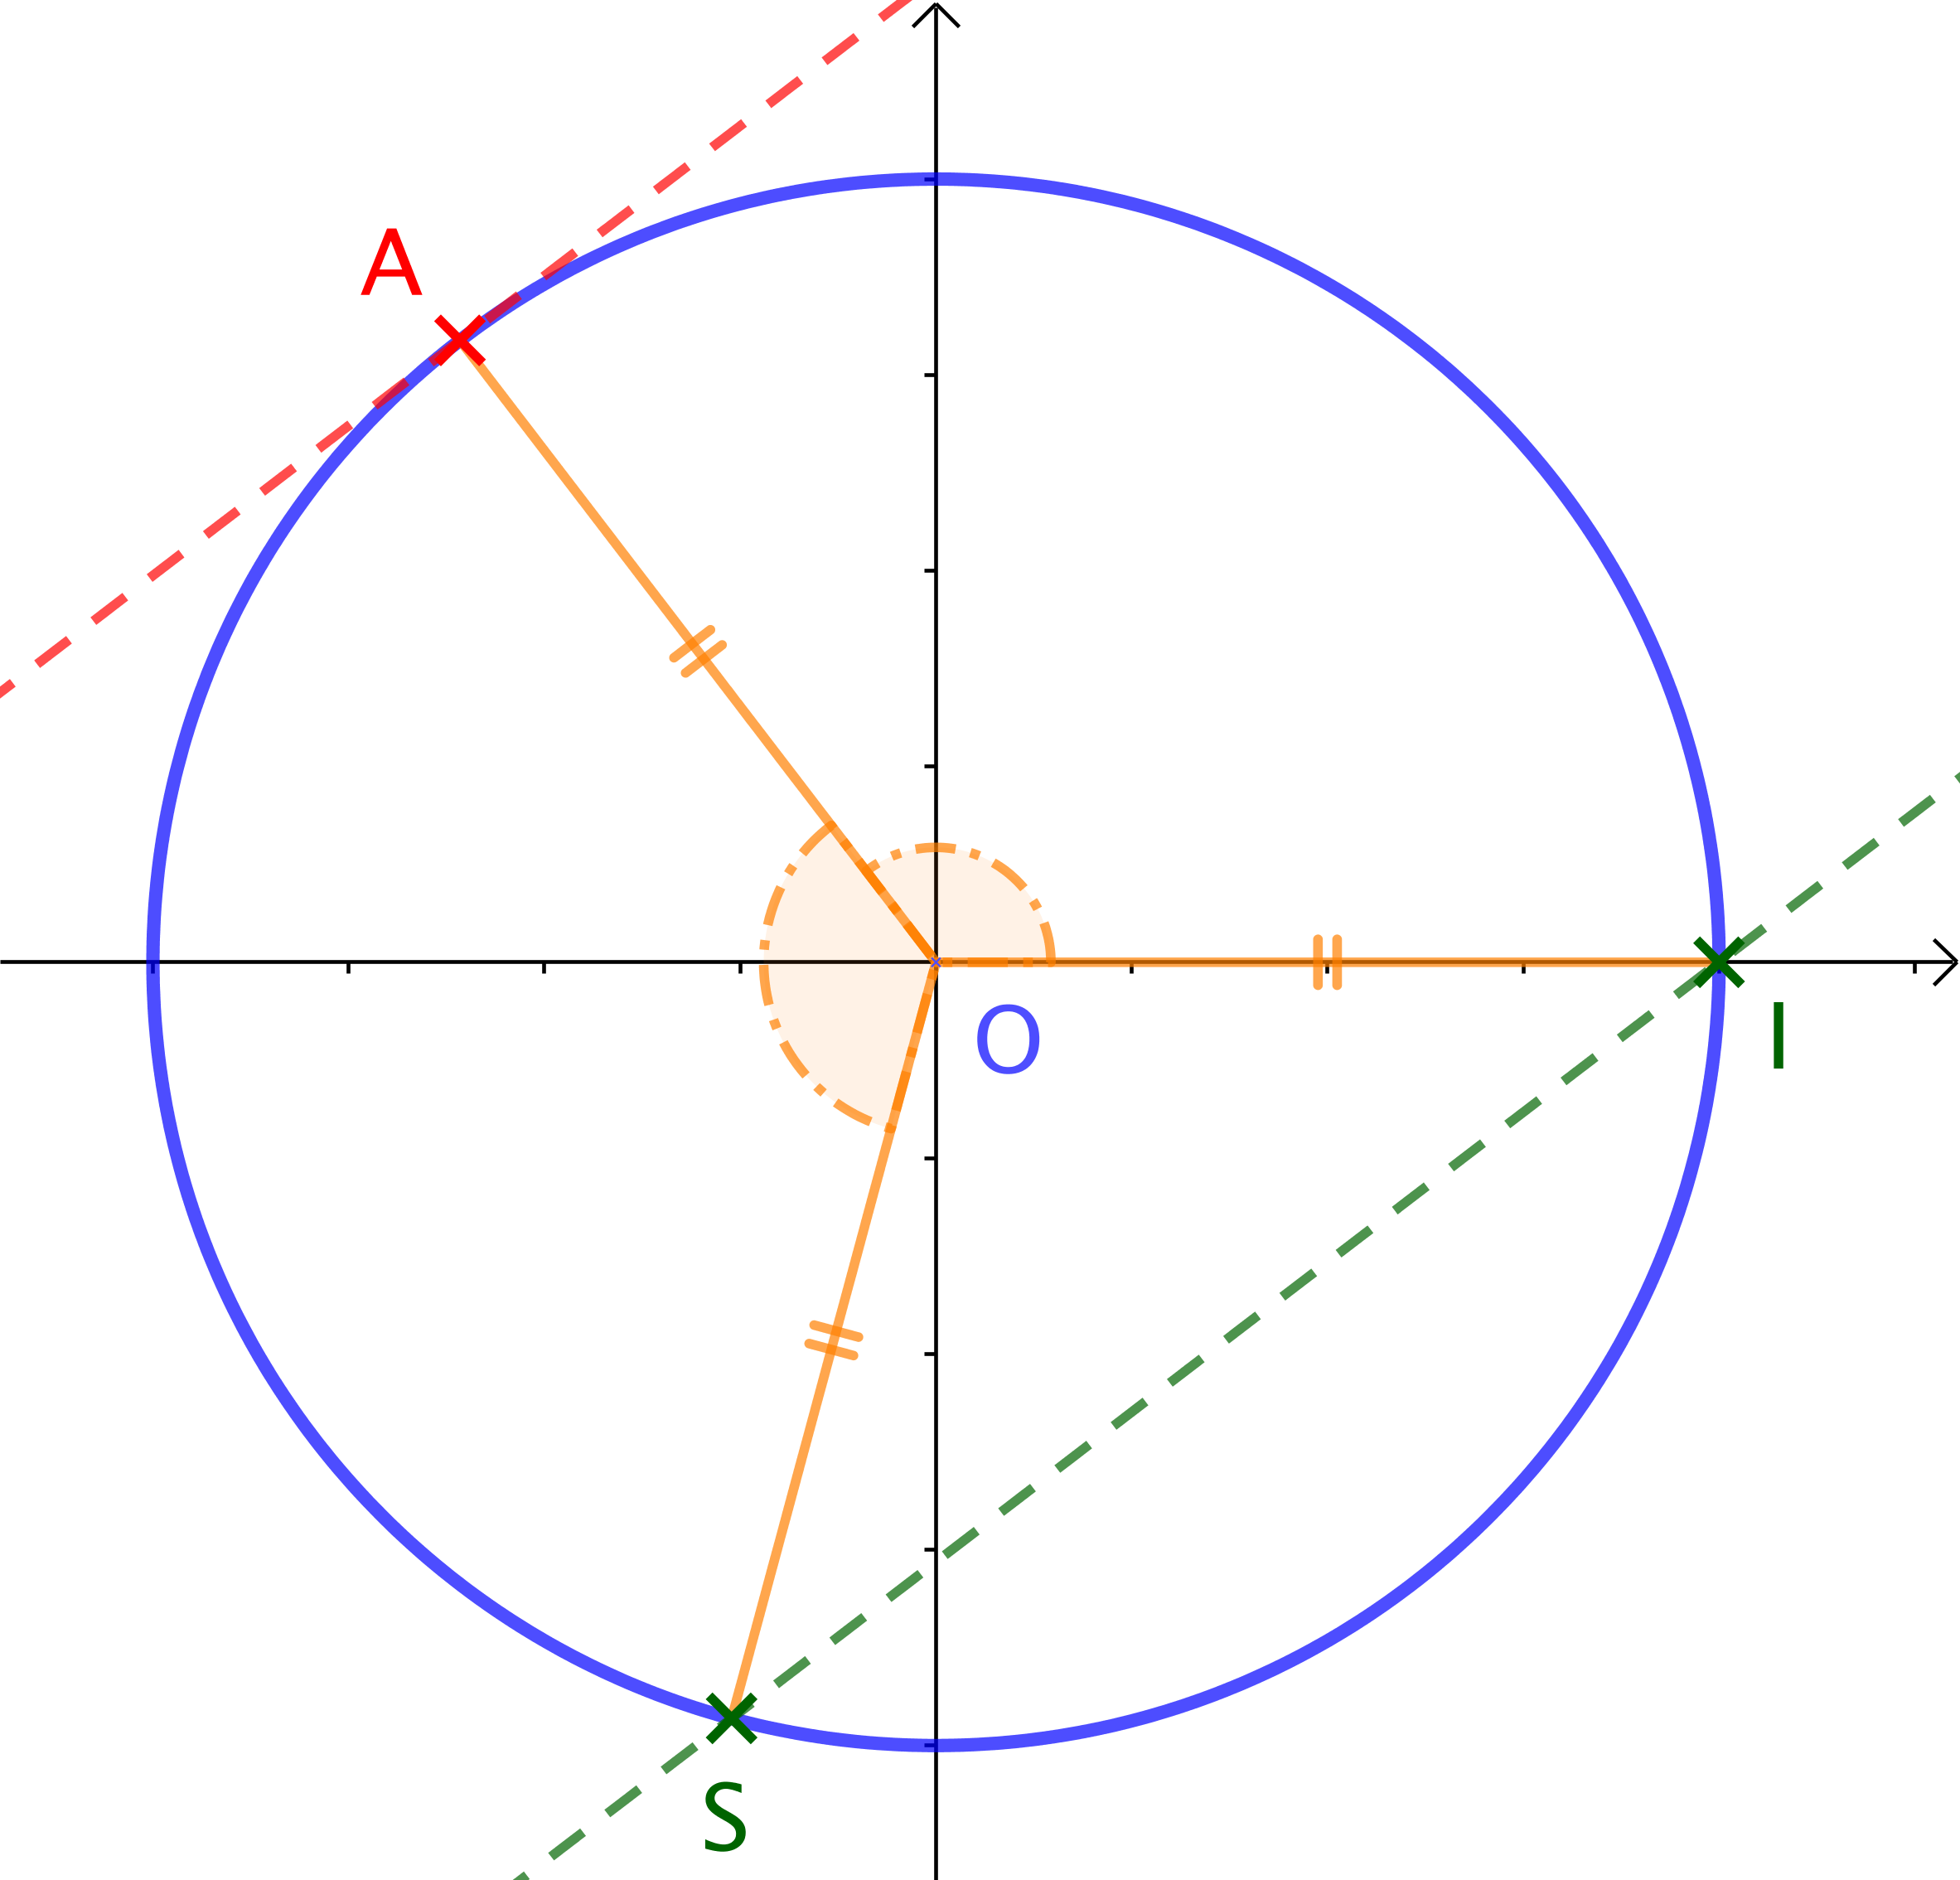
\includegraphics[scale = .75]{addition-on-ellipsis/proof/rotation-A-is-B.png}}
\end{center}
\smallskip

Il est immédiat que
$\angleorient{\vect{OI}}{\vect{OA}}
= \angleorient{\vect{OA}}{\vect{OS}}$
puis que
$- \angleorient{\vect{AO}}{\vect{OI}}
= \angleorient{\vect{AO}}{\vect{OS}}$ .
Nous en déduisons que la droite $(AO)$ est la bissectrice du triangle isocèle $SOI$  issue du sommet principal de ce dernier d'où $(AO) \,\bot\, (SI)$ puisque cette bissectrice particulière est aussi une hauteur. Il est alors clair que $(SI)$ est parallèle à la tangente en $A$ au cercle.



% ------------- %


\section{\texorpdfstring{Toute ellipse d'équation $(x(t) , y(t)) = (x_0 + a \cos t , y_0 + b \sin t)$ est un groupe}%
                        {Toute ellipse d'équation (x(t) , y(t)) = (x0 + a cos t , y0 + b sin t) est un groupe}}
      
Dans les preuves des sections précédentes, on constate que la construction géométrique se traduit par une identité basique qui est la clé de la périodicité de la suite de points $\left( A_i \right)$ . 
\begin{enumerate}
	\item Pour le cercle, c'était $\theta_i + \theta_{i+1} = \theta_{i+3} + \theta_{i+4}$ avec $\theta_i = \vangleorient{OI}{OA_i}$ . Nous nous intéressons ici juste à la 2\ieme preuve donnée dans la section \ref{circle-proof-2}. 

	\item Pour la parabole, c'était $x_i + x_{i+1} = x_{i+3} + x_{i+4}$ avec $x_k \in \RR$ des abscisses. 

	\item Pour l'hyperbole, c'était  $x_i x_{i+1} = x_{i+3} x_{i+4}$ avec $x_k \in \RRs$ des abscisses.
\end{enumerate}


\medskip


En fait, si $\Gamma$ désigne une ellipse, une parabole quelconque, ou une hyperbole quelconque, on peut démontrer l'existence d'un point $E \in \Gamma$ tel que la construction qui à $A \in \Gamma$ et $B \in \Gamma$ associe le point $S$ tel que $\setgeo*{C}{AB} \,/\!/\, \setgeo*{C}{ES}$ définisse une loi de groupe $\star$ sur $\Gamma$ avec $E$ pour élément neutre. 
Les cas étudiés dans ce document n'en sont que des cas particuliers. 
Le lecteur intéressé peut se reporter à  
\emph{\og Faire des additions modulaires sur une ellipse \fg} ,
\emph{\og Faire des additions sur une parabole \fg} 
et
\emph{\og Faire des produits sur une hyperbole \fg}
qui ont été rédigés par l'auteur de ce document
\footnote{
	Voir \texttt{addition-on-ellipsis.pdf} , \texttt{addition-on-parabolas.pdf}  et \texttt{product-on-hyperbolas.pdf}  à l'adresse \url{https://github.com/bc-writing/drafts} .
}.


\medskip


Tout comme dans la preuve dans la section \ref{circle-proof-2} , on constate alors que la construction \emph{\og magique \fg} est telle que $\forall n \in \NN_{\geq 5}$ , $A_{n}$ est l'unique point de $\Gamma$ tel que $\setgeo*{C}{A_{n} A_{n-1}} \,/\!/\, \setgeo*{C}{A_{n-3} A_{n-4}}$ . On en déduit alors que $A_{n} \star A_{n-1} = A_{n-3} \star A_{n-4}$ . On retombe alors sur une identité similaire à celles redonnées ci-dessus mais avec la loi $\star$ au lieu des lois $+$ avec des angles orientés, $+$ avec des réels et $\times$ avec des réels non nuls. On conclut alors de la même façon. Que les mathématiques sont belles quand on prend le temps de les écouter !


\end{document}
